\documentclass[11pt,a4paper,twoside,notitlepage,openright]{report}
%\usepackage[utf8]{inputenc}
\usepackage{amsmath}
\usepackage{amsfonts}
\usepackage{amssymb}
\usepackage{graphicx}
\usepackage{subfig}

\usepackage{hyperref}
\hypersetup{hidelinks}
\usepackage{frontespizio}
\usepackage[english]{babel}
\usepackage{outlines}
\usepackage[output-decimal-marker={.}]{siunitx}
\usepackage{physics}
\usepackage{xcolor}
\usepackage{slashed}
\usepackage{amssymb}

\usepackage[left=2cm,right=2cm,top=2cm,bottom=2cm]{geometry}
\usepackage[toc,page]{appendix}
\usepackage[compat=1.1.0]{tikz-feynman}
\usepackage{wrapfig}
\usepackage{graphicx, wrapfig}
%\usepackage[rightcaption]{sidecap}
\usepackage{sidecap}
\usepackage{comment}

\tikzfeynmanset{every blob = {minimum size = 3mm}}
\newcommand{\commento}[1]{}
\newcommand{\Lagr}{\mathcal{L}}
%{\bfseries #1 \medskip}
\newcommand{\transv}{transverse asymmetry }
\pagestyle{headings}
\sidecaptionvpos{figure}{t}
%\setlength\intextsep{2pt}
\setlength{\textfloatsep}{10pt plus 1.0pt minus 1.0pt}
\author{Adriano del Vincio}


%frontespizio tesi
\begin{document}
\begin{frontespizio}
\Logo[2.5cm]{Simbolo/cherubino_pant541.eps}
\Istituzione{Università di Pisa}
\Dipartimento{Fisica "Enrico Fermi"}
\Corso[Laurea]{Fisica}
\Titoletto{Tesi di laurea}
\Titolo{Commissioning and first data analysis \\ of the Mainz radius experiment.}
\Candidato[562946]{Adriano Del Vincio}
\Relatore{Prof. Francesco Forti \\ Prof.ssa Concettina Sfienti}
\Annoaccademico{2022-23}
\end{frontespizio}

\title{Commissioning and first data analysis of the Mainz Radius Experiment.}
\date{} 
\tableofcontents
\listoffigures
\listoftables
% Capitoli tesi
\include{Abstract/abstract}

\chapter{Physics Motivation for Neutron Skin Thickness Measurement} \label{intro}
\commento{
\begin{itemize}
\item explain neutron skin thickness.
\item connection to neutron stars radious, and neutron stars description.
\item Equation of state (EoS) for high density nuclear matter.
\item Parity-violating scattering experiment for extracting neutron skin thickness.
\item mention the weak form factor.
\item Transverse asymmetry as background for Parity-violating experiment. 
\item Mention the other experiment, like PREX, that measure zero $A_{n}$ for Lead.
\end{itemize}}

\section{The Mainz Radius Experiment}

The Mainz Radius Experiment (MREX), at the Mainz nuclear physics institute, is an experimental campaign with the aim of investigating the complex nature of atomic nuclei. The strong force, whose presence was first speculated by Yukawa in 1935, is responsible of a broad range of phenomena: from characteristic of atomic nuclei, the compositions of baryons and meson to the exotic structure of Neutron stars. So, the field of nuclear physics provides many answers to fundamental questions in other fields of physics. In particular the neutron stars, that are one of most interesting astrophysical object in the universe, are ideal to study and test theories of dense matter, providing so many connection between particle physics, astrophysics and nuclear physics. It can be surprising to think that, despite a difference of so many order of magnitude, neutron rich nuclei and neutron stars have the same basic physics, enshrined by the the Equation Of State (EOS) of neutron rich matter. The Equation Of State represents the fundamental relation between the state variables as temperature, energy, pressure and neutron-proton asymmetry. Specifically, the final goal of the MREX experiment is to determine an important parameter of the EOS, that is the slope of the symmetry energy at saturation density $L$. This parameters is important for the determination of the radius of the neutron stars, but it is also responsible of a peculiar characteristic shown by heavy nuclei: the neutron skin thickness $\delta r_{np}$. The neutron skin thickness is a phenomena that affect heavy nuclei which consists in the accumulation of the excess of neutrons near the surface of a nucleus. Such skin thickness is strongly sensitive to $L$, so an accurate determination of the neutron skin provides significant constrains on the value of $L$ which in turn is used as an input to many theoretical models of the structure of the neutrons stars.
The determination of $\delta r_{np}$ presents considerable difficulties. While $r_{p}$ is known with high accuracy, thanks to the electrons elastic scattering experiment which involves electromagnetic force, the determination of $r_{n}$ has traditionally relied on hadronic experiments which involves proton-nucleus scattering, $\pi^{0}$ photo-production, $\alpha$ and $\pi$ nucleus scattering. Those process suffer from large and often uncontrolled theoretical uncertainties that compromises the extraction of the neutron density. The most promising method, that is the least model dependent, is the parity-violating electron scattering. In this reaction longitudinal polarized electrons are elastically scattered off unpolarized target. This method consist in the measurement of the asymmetry between right and left handed electrons:

\begin{equation}
A_{pv} = \dfrac{\sigma_{R} - \sigma_{L}}{\sigma_{R} + \sigma_{L}}
\end{equation}

This process is dominated by the exchange of a virtual photon, which is sensitive to charge form factor, and a $Z_{0}$ boson, that is sensitive to the weak form factor. Because of the fact that the weak charge of the neutrons is $Q_{w} = 0.99$ and the weak charge of the proton is $0.04$, the weak form factor contains the information on the neutron density, necessary to measure $\delta r_{np}$. The MREX experiment will measure the neutron skin thickness via the parity violating scattering at the new MESA accelerator.

\section{Nuclear Equation of State (EOS) and Neutron Skin Thickness}

\commento{In this section we have to explain what is the neutron skin thickness and why this parameter is related to the Equation of State for nuclear matter (in particular, the slope of the Symmetry energy in the semiempirical mass formula). Then, explain the parallelism between Neutron stars and Nuclear matter (the share the same EOS), and underline the relation between radius of the neutron stars and EOS.}

During the 30s of the last century, a considerable part of the scientific community was concentrated in the study of the structure of atomic nuclei. The discovery that every atoms has a positive charged nucleus dates back to 1908, with the famous Rutherford experiment, where alpha particles scatter from a thin gold foil. In the following years, especially with the birth of quantum mechanics in the second half of the 1920s, significant progress were made in the knowledge of atomic nuclei and their properties. In 1935, a significant contribution was given by Carl Friedrich von Weizsäcker, that proposed the semi-empirical mass formula, to approximate the mass of an atomic nucleus. Although some refinements have been made over the years, the general structure of the formula is the same today. 
The model proposed by Weizsäcker is the application of the liquid-drop model for nuclear matter, where the Nucleus is described as drop of protons and neutrons, that are assumed to be incompressible and are held together by a nuclear potential. The semi-empirical mass formula states that the mass of a nucleus is given by 

\begin{equation}
m = Zm_{p} + Nm_{n} - \frac{E_{B}(N,Z)}{c^{2}}
\end{equation}

An important terms is the binding energy $E_{B}$, that contains 5 parameters:

\begin{equation}
E_{B} = a_{V}A -  a_{s}A^{\frac{2}{3}} - a_{c}\dfrac{Z^{2}}{A^{\frac{1}{3}}} -a_{asym}\dfrac{(N - Z)^{2}}{A} + \delta(N,Z)
\end{equation}

The first two terms $a_{V},a_{s}$ are taken from the liquid drop model, and are the volume energy and the surface energy. The volume term represent the energy due to the interaction of each nucleon with the other nearby nucleons. This term is proportional to $A$, that is the number of nucleon of the nucleus, which is proportional to the volume, hence the name. The second term represent is the surface energy, and it is a correction to the volume energy. The volume energy assume that each nucleon interact with a constant number of nearby nucleons, but this is not true if we consider the external protons and neutrons, because they have less neighbors to interact with. This correction terms is then proportional to $A^{\frac{2}{3}}$, that is the also proportional to the surface area. 
The third term $a_{c}$ denote the binding energy correction due to the repulsion between protons. The fourth term is $a_{asym}$, the asymmetry term, and it is proportional to the asymmetry between neutrons and protons. The theoretical justification for this terms is due to the Pauli exclusion principle. Neutrons and protons are distinct type of particles, and occupy different quantum states. Because neutrons/protons are fermions, they can't occupy a state with the same quantum numbers, therefore higher energy states are progressively filled. If there is an asymmetry between neutrons and protons, for example the number of neutrons is greater than the number of protons, some neutrons will be in higher energy states respect to the protons. The imbalance between the nucleons causes the energy to be higher respect to the situation with the same number of protons and neutrons. 
The last term the pairing term, and describes the effect of spin coupling, and has positive/negative values for even or odd N,Z. 
We want to focus on the fact that the liquid-drop model has the underlying assumption that the nucleons are incompressible. Because of this it is well defined the concept of saturation density, the fact that the density, at first order, is almost constant and independent of mass number A.
In the context of neutron stars, it is more useful to take the thermodynamic limit in which the number of nucleons and Volume are taken to infinity. The binding energy per nucleons can be written as:

\begin{equation}
\epsilon (\rho_{0}, \alpha) = -\frac{E_{B}}{A} = -a_{V} + a_{asym} \dfrac{\rho_{n} - \rho_{p}}{\rho_{n} + \rho_{p}}
\end{equation}

In reality, this simple equation is only an approximation, because the nuclear matter doesn't behave like an ideal liquid drop, and it is not incompressible. To describe the response of the nuclear matter to density variation, as well as temperature, etc... we need the equation of state (EOS) of the system, that binds these quantities thermodynamically. For neutron stars, the EOS depends on $\rho$, the conserved baryon density, and neutron-proton asymmetry $\alpha$, in the ideal limit of $T = 0$:

\begin{equation}
\epsilon (\rho,\alpha) = \epsilon_{snm} (\rho, \alpha = 0) + \alpha ^{2} S(\rho) + O(\alpha ^{4})
\end{equation}

The energy density is expanded in a power series of $\alpha = \dfrac{\rho_{n} - \rho_{p}}{\rho_{n} + \rho_{p}}$. No odd power of $\alpha$ appears in the expansion, because the strong force doesn't depend on the isospin, or in other words, neglecting electromagnetic interaction and weak interaction, the equation of state depends only on the relative asymmetry between neutrons and protons, it doesn't matter if such an asymmetry is biased towards protons or neutrons.
The terms $S(\rho)$ is the symmetry energy, and it represents the cost of converting symmetry nuclear matter ($\alpha = 0$) to pure neutrons matter, as the case of neutron star. Now we can proceed considering the saturation density. A further expansion around the saturation density $\rho$ is necessary:
	
\begin{equation}
\begin{split}
S(\rho) &= J + L \cdot \dfrac{\rho - \rho_{0}}{3 \rho_{0}} + \dfrac{1}{2} K_{sym} \cdot \biggl(\dfrac{\rho - \rho_{0}}{3 \rho_{0}}\biggl)^{2} \\
\epsilon _{smn} (\rho) &= \epsilon_{0} + \dfrac{1}{2}K_{0} \biggl(\dfrac{\rho - \rho_{0}}{3 \rho_{0}} \biggl)^{2} 
\end{split}
\end{equation}

Several new terms appear in this expression:
\begin{itemize}
\item $\epsilon_{0}$ is the energy per nucleon for symmetric matter at saturation density.
\item $J$ is the symmetry energy at saturation density.
\item $L$ is the slope of the symmetry energy.
\item $K_{0}$ is the incompressibility coefficient for symmetry matter. 
\item $K_{sym}$ is the incompressibility coefficient for the symmetry energy.
\end{itemize}

In this expression appears for the first time $L$, the slope of the symmetry energy. This is a key component of the EOS, whose values is an important parameter to determine the radius of neutron star. $L$ quantifies the difference between the symmetry energy at saturation (as in the nuclear core) and the symmetry energy at lower densities, as in the nuclear surface.$L$ is also related to the pressure $P$ at saturation density. Giving the EOS in term of $\rho,\alpha$, the pressure is given by:

\begin{equation} \label{eq:Pressure}
P = \rho^{2} \dfrac{\partial \epsilon(\rho, \alpha)}{\partial \rho}
\end{equation} 

A formal demonstration of this relation is given in the appendix (\commento{mettere referenza}). We know write $\epsilon_{snm}$ making explicit all the dependencies:

\begin{equation}
\epsilon (\rho, \alpha) = (\epsilon_{0} + \alpha^{2} J) + \alpha^{2}Lx + \frac{1}{2} (K_{0} + \alpha^{2}K_{sym})x^{2}
\end{equation}

we substitute $x = \dfrac{\rho - \rho_{0}}{3 \rho_{0}}$. Considering pure neutron matter $\alpha = 1$, the pressure at saturation density $P_{0}$ can be easily computed withe the formula (\ref{eq:Pressure}). The result is the following:

\begin{equation}
P_{0} \simeq \dfrac{1}{3}\rho_{0} L
\end{equation}

From this expression we learn that the slope of the symmetry energy is essential to determine the pressure for densities near saturation. The contribution of the symmetric term $\epsilon_{snm}(\rho)$ vanishes, and at first order the pressure depends only on $L$. Because of this, it becomes more and more clear the link between $L$ and the neutron skin thickness. Let's consider the case of the $^{208}Pb$, with ad excess of 44 neutrons. Placing the excess of neutrons in the surface of the nucleus is discouraged by surface term $a_{S}$, which tends to minimize the area. However, if the excess of neutrons is placed in the core of the nucleus, this is increase the symmetry energy $S(\rho)$. In the end the neutron skin is the result of the competitions between the surface tension and the slope of the symmetry energy.
 Measurement of the neutron skin have been performed by the PREX collaboration at Thomas Jefferson National Accelerator Facility in Virginia \cite{Abrahamyan:2012gp}, however the precision attained was insufficient to distinguish between the various competing models which describe the relation between $\delta r_{np}$ and $L$ (\ref{fig:LvsR}). Despite this, theoretical predictions states that there is a strong correlation between these two quantities, in the following plot we show how different theoretical models, with different values of $L$ used as input, predict the values of $\delta r_{np}$ for lead:

\begin{figure}[hbtp]
 \centering
 \includegraphics[width=0.75\textwidth]{Introduzione/LvsR.pdf}
 \caption{Neutron skin thickness of $^{208}Pb$ as a function of the slope of the symmetry energy $L$. The error bars represent $\pm \SI{0.06}{\femto \meter}$ and $\pm \SI{0.03}{\femto \meter}$ for the future experiments of PREX-II and MREX. Notice the different scale for x and y axis: the uncertainty for the neutron skin measurement is amplified for the correspondent values of $L$ }
 \label{fig:LvsR}
 \end{figure}
 
A strong linear correlation is evident, and so it is clear that measuring the neutron skin is a promising way to measure $L$. 

\subsection{Neutron Star Radius}


\section{Parity-violating Scattering Experiment}

The parity violating electron scattering seems to be the most promising method in order to determine the neutron-skin thickness for $^{208}Pb$. The choice of lead is due to the significant neutron excess and stability of lead nuclei ($^{208}Pb$ is a double magic nucleus). The advantage of this method is that it is free from the many uncertainties associated to strong interaction. The main disadvantage is the necessity to accumulate large statistics, because the reaction are mediated by the weak interaction, that produce a smaller amplitude compared to electromagnetic and strong interaction. 
The parity violating scattering is high sensitive to the neutron density because, as mention above, the weak charge of the neutron is higher compared to the weak charge of the proton.
In this reaction, longitudinally polarized electrons are elastically scattered off a lead target. The important quantity to determine is the parity violating asymmetry $A_{PV}$, the difference in cross section between the scattering of right and left handed electrons. 

\begin{equation}
A_{PV} = \dfrac{\sigma_{R} - \sigma_{L}}{\sigma_{R} + \sigma_{L}}
\end{equation} 

The theoretical calculation of $A_{PV}$ concern the interference between the exchange of virtual $\gamma$ and $Z^{0}$. In the Born approximation $A_{PV}$ is directly proportional to the weak form factor, and it is given by the formula below:

\begin{equation}
A_{PV} \simeq \dfrac{G_{F} Q^{2}}{4 \pi \alpha} \cdot \dfrac{Q_{W} F_{W}(Q^{2})}{Z F_{ch}(Q^{2})}
\end{equation} 

$G_{F}$ is the Fermi constant, $Q^{2}$ is the transferred momentum, Z and $Q_{W}$ is the electric and weak charge of the nucleus. The Charged form factor of the lead nucleus is known with high accuracy (precision of 0.02 \%), so in this limit the only quantity that is unknown is $F_{W}(Q^{2})$. In the long wavelength approximation, the weak form factor at single value of momentum transfer is given by:

\begin{equation}
F_{W}(Q^{2}) = \frac{1}{Q_{W}} \int \rho_{W}(r) \dfrac{sin(Qr)}{Qr} d^{3}r = (1 - \frac{Q^{2}}{6} R^{2}_{W} + \frac{Q^{4}}{120}R^{4}_{W} + ...)  
\end{equation}

The form factor is normalized in such a way that $F_{W}(Q^{2} = 0) = 1$. The weak charge radius correspond to $R^{2}_{W} = -6 \frac{\partial F_{W}}{\partial Q^{2}}\Bigr|_{\substack{Q^{2} = 0}}$. Now it is clear that parity-violating experiment are a promising method to extract information about neutron density. The effort is represented by the small values of $A_{pv}$ asymmetry. Typical values are on the order of $1 \, ppm$ or less, for lead target. This requires high statistic to reduce the uncertainty of the measurement. 
In 2012 PREX collaboration measured for the first time through parity-violating experiment the neutron skin, the values is:

\begin{align*}
\delta r_{np} = 0.33^{+0.16}_{-0.18} \SI{}{\femto \meter}
\end{align*}

The error associated to this first measurement is not enough small to provide significant constraints on the values of $L$. Because of this, the MREX experiment has the objective of measuring the neutron radius of lead with a precision of $0.5 \%$  ($\pm \SI{0.03}{\femto \meter}$). This high precision is needed to decrease the uncertainty associated to L. For example, the left plot in \ref{fig:LvsR}, shows the correlation between the neutron skin thickness of $^{208}Pb$ and the slope of the symmetry energy as predicted by FSUGold model (\cite{Fattoyev_2011}). With a precision of $\pm \SI{0.03}{\femto \meter}$, $L$ is determined with $\pm \SI{12.1}{\mega \electronvolt}$.

\section{Transverse Asymmetry}

\commento{Here we have to introduce the aim of this thesis: the transverse asymmetry is a source of background for the parity-violating experiments. Furthermore the theory is not working well for some nuclei ($^{208}Pb$), so mention PREX paper about the last measurement on carbon and lead, the problem that they measure $0$ transverse asymmetry.}

The parity-violating scattering has numerous advantages for extracting the neutron-skin thickness of nuclei. However, the asymmetry to measure is rather small. The important effort is to reduce at most possible systematic effects that can alter the result of the measurement. One of the principal source of background for the measurement of $A_{PV}$ is a different process that concerns transverse polarized electrons. The different polarization of the electrons produce an asymmetry that is called beam normal single spin asymmetry, or transverse asymmetry $A_{n}$. Because such asymmetries are typically one order higher that the parity-violating ones, a small normal component of the beam polarization during parity-violating experiment can produce a systematic effect that alter the final result. The subject of this thesis is the measurement of transverse asymmetry $A_{n}$ for carbon target, performed at MAMI, the Mainz microton accelerator. The choice of carbon target is due to the fact that the transverse asymmetry for carbon is well known and already measured at MAMI; the expected asymmetry is roughly $20 \, ppm$ , thus it is particularly suited for a commissioning of the new experimental setup. In this section don't introduce physics of this process, that will be extensively treated in the next chapter. However, we mention that such measurement are challenging because they require calculation of box diagrams with intermediate excited states \cite{Gorchtein_2008}.
After the determination on $A_{n}$ for $^{12}C$, the next step of the MREX experiment will be the determination of the \transv for $^{208}Pb$. As already mentioned, this is mandatory to constrain the systematic effects of PV experiment. However, it is also interesting because for last measurement performed by PREX \cite{HAPPEX:2012fud} the \transv for $^{208}Pb$ target is compatible with zero, and this is in striking disagreement with the theoretical predictions. 


\chapter{Transverse Asymmetry} \label{transv}

\paragraph{}
This chapter is focused on describing the theory behind the \transv . The \transv arises from interference between two scattering amplitudes and it is deeply connected with the Time-reversal operator. These two contributions due to the electromagnetic interaction between the incident electron and the nucleus are explained by showing what are the limits of current theory and what are the most important terms in theoretical prediction. The chapter ends by presenting the problem of the anomalous observation made by PREX of zero transverse asymmetry and a study on the accuracy with which it is possible to measure the asymmetry. 

\section{Description of the Process}

The Beam Normal single spin asymmetry, which we will refer for brevity as Transverse asymmetry, originates from the interference of two scattering process. The theory of the electron scattering against a spin $0$ target is extensively treated in \cite{Gorchtein_2008}.
To understand why the interference of this two scattering amplitude give rise to an asymmetry, we first have to look at the kinematic of the experiment:  \newline

\begin{figure}[hbtp]
\centering
\includegraphics[width = 0.6\textwidth]{Transverse/scattering.pdf}
\caption{Scheme of the scattering process. In blue the incident electron and nucleus, in red the outgoing electron and nucleus. All the quantities are referred to the center of mass frame. The small arrow over the vector represent the electron spin, aligned in the normal plane.}
\end{figure}

Where all the momenta are measured respect to the center of mass frame. In the figure we can confront the two situation before and after applying the Time-reversal operator, $\hat{\Theta}$. Looking at the picture we can understand that : 

\begin{itemize}
\item Before applying $\hat{\Theta}$, we have the incident electron with $\vec{k}$ momenta and the nucleus with $\vec{P}$ momenta, after applying $\hat{\Theta}$ we have that the incident/outgoing electron and the incident/outgoing nucleus are exchanged.
\item The $\hat{\Theta}$ operator acts also on the spin of the electron. Because we are considering process where the spin doesn't flip, the two situations are not equivalent.
\item Considering that the process is elastic, the kinematic is the same, taking $\vec{p}$ and $\vec{k}$ as the initial particle momenta, or $\vec{p}'$ and $\vec{k}'$. 

\end{itemize}

The time-reversal operator seems to connect the two different cases of UP and DOWN polarized electron. Our effort is to measure the asymmetry between the two cross section:

\begin{equation}
A = \frac{\sigma_{\uparrow} - \sigma_{\downarrow}}{\sigma_{\uparrow} + \sigma_{\downarrow}}
\end{equation}

And it's particularly clear that a non-zero asymmetry depends on how the time-reversal act on the elastic amplitude of the process. \\
With this idea, let's see in more detail the $\hat{\Theta}$. We know that $\hat{\Theta}$ is an anti-unitary operator that can be always seen as:

\begin{align*}
\hat{\Theta} = U \cdot K
\end{align*} 
Where $U$ is an unitary operator, while $K$ is the complex conjugation operator that generates the complex conjugate of each coefficient in front of it. If we consider a ket describing a system we have that:

\begin{equation}
Kc \ket{\alpha} = c^{*} K \ket{\alpha}
\end{equation}

Now, let's consider $H$ as the hamiltonian of our system. We want to apply the $\hat{\Theta}$ operator. We can now use the assumption that the hamiltonian consist of two term, which correspond to the two different scattering process. Because of the electromagnetic interaction conserve $CP$, so also $T$ is conserved, we know in advance that each piece of the hamiltonian commute with $\hat{\Theta}$. Now let's see what happen for an hamiltonian which has an imaginary part:

\begin{equation}
H = H_{R} + i H_{Im} \quad ; \quad \hat{\Theta} H \hat{\Theta}^{-1}= \hat{\Theta}H_{R} \hat{\Theta}^{-1} + \hat{\Theta} i H_{Im} \hat{\Theta}^{-1} \Rightarrow H_{R} - i H_{Im} \neq H
\end{equation}

what we understand from these simple calculation is that to give rise to an asymmetry, we expect an imaginary part of the scattering amplitude different from zero.\\
At the $\alpha$ leading order, the two process of the electron-Nucleus scattering that give rise to the asymmetry involve the exchange of one-photon-exchange (OPE) and two-photon-exchange (TPE). The Feynman diagrams that describes the processes are the following: 

\begin{figure}[hbtp]
\[
\feynmandiagram [scale = 1, transform shape][baseline = (h), horizontal = d to j]{
	a [particle = \(e^{-}\)] -- [fermion, thick] c -- [fermion, thick ] f -- [fermion, thick] g [particle = \(e^{-}\)],
	c -- [photon, edge label = \(\gamma\)] d [blob],
	f -- [photon, edge label = \(\gamma\)] j [blob],
	h [particle = \(C^{12}\)]-- d -- [fermion, thick] j -- k [particle = \(C^{12}\)] ,
	};
\qquad \qquad \qquad
\feynmandiagram [scale = 1, transform shape][ vertical = c to d]{
	a [particle = \(e^{-}\)] -- [fermion, thick] c -- [fermion, thick] g [particle = \(e^{-}\)],
	c -- [photon, edge label' = \(\gamma\), momentum = {[arrow style = red]\(k\)}] d [blob],
	h [particle = \(C^{12}\)] -- [fermion, thick] d -- [fermion, thick] j [particle = \(C^{12}\)],
	};
\]
\caption{TPE and OPE diagrams in electron nucleus scattering.}
\label{fig:FeynmannDiagrams}
\end{figure}

The important quantity to compute the cross section is the scattering amplitude. The scattering amplitude is given by the two contributions: the exchange of a single virtual photon $A_{1}$ and the terms given by the two photon exchange $A_{2}$. In general we can write that the total scattering amplitude $S$:

\begin{equation}
S = \dfrac{e^{2}}{Q^{2}} \overline{u}(k') [ \, m_{e} A_{2} + A_{1} \slashed{P} \,] \overline{u}(k)
\end{equation}

Where in this expression $\vec{P} = \frac{\vec{p} + \vec{p}'}{2}$. The second term $A_{1}$ has a simple expression, given by the form factor of the nucleus:

\begin{align*}
A_{1} = 2Z F_{N}(Q^{2})
\end{align*} 

This expression is obtained if we look at the \ref{fig:FeynmannDiagrams}. For the one photon exchange the first vertex connects the incident and scattered electron, whose expression is given by $-ie \gamma^{\mu}$. The second vertex connect the carbon nucleus with the virtual photon. The carbon is threated like as a spin $0$ particle, and the contribution due to the charge density in enshrined in the form factor. The lagrangian term for a vertex of this type is given by the formula: 

\begin{equation}
\Lagr_{interaction} = +ieA_{\mu}(\Phi \partial^{\mu} \Phi^{\dag} - \Phi^{\dag}\partial_{\mu} \Phi)
\end{equation}

For the spin 0 field $\Phi$. This is not the only piece of the lagrangian: there exist another term of interaction, that involves a vertex with four particles which is not of our interest. This interaction term give rise to the Feynmann rule for spin 0 particle, and we have to substitute for this vertex:

\begin{align*}
-ie(p + p')_{\mu}
\end{align*} 

And we recognize, apart from a factor 2, $\slashed{P}$ which multiplies $A_{1}$. The last term is the feynmann propagator for the photon, that give the $\frac{1}{Q^{2}}$ term. This first part of the scattering amplitude is T-even, and it is purely real, so it is the imaginary part of the two photon exchange which give rise to the asymmetry. The expression that connects the amplitude with the \transv is given by:

\begin{equation} \label{eq:integral}
A_{n} = -\frac{m_{e}}{\sqrt{s}} tan \bigl (\frac{\theta_{CM}}{2} \bigl) \dfrac{\Im(A_{2})}{ZF_{N}(Q^{2})}
\end{equation}

Looking at this formula, the theoretical effort to compute the transverse asymmetry is given by the imaginary part of $A_{2}$. The calculation of this quantity is theoretically challenging, due to the fact that at energies of $\simeq \SI{1}{\giga \electronvolt}$ of incident electrons, contributions from intermediate excited states become important. Because of this, the contribution of $A_{2}$ are given by the sum of elastic intermediate state and inelastic terms, which involve hadronic excitations.

\subsection{Hadronic Tensor}

The imaginary part $A_{2}$ is related to the two-photon exchange. To compute this quantity, we have to perform an integration over the internal momenta of the electron $k_{1}$ (see figure \ref{fig:FeynmannDiagrams}). This contribution, following \cite{Gorchtein_2008}, is given by:

\begin{equation}
\Im(A_{2}) = e^{4} \frac{1}{(2\pi)^{2}} \int \dfrac{l_{\mu \nu} \cdot W^{\mu \nu}}{2E_{1} Q_{1}^{2} Q_{2}^{2}} d^{3}\vec{k_{1}}
\end{equation}

Two new terms appear in this expression. The first term is $l_{\mu \nu}$, named leptonic tensor. This term is given computing the Amplitude for the upper part of the diagram, which involve the incident and scattered electron:

\begin{equation}
l_{\mu \nu} = \overline{u}(k') \gamma_{\nu} (\slashed{k}_{1} + m_{e}) \gamma_{\mu} u(k)
\end{equation}

In this expression is immediate to recognize the feynmann rules for fermion vertex. The term $(\slashed{k_{1} + m_{e}})$ comes from the fermion propagator of the internal electron, which is:

\begin{align*}
\dfrac{i(\slashed{p} + m)}{p^{2} + m^{2}}
\end{align*}

The other term is $W^{\mu \nu}$, the hadronic tensor. For the elastic contribution this term is simply given by the feynmann rules for vertex with spin 0 particles, with the proper correction of the form factor, so we can write:

\begin{equation}
W_{\mu \nu} = \pi \delta((p + k - k_{1})^{2} - M^{2}) (2p + q_{1})_{\mu} (2p' + q_{2})_{\nu} \times Z^{2} F_{N}(Q_{1})  F_{N}(Q_{2})
\end{equation}

At this point, one can substitute in the integral above, and compute the contribution of the transverse asymmetry due to the elastic term. This first terms scales with the nuclear charge $Z\alpha$, and this is important for electron scattering with heavy nuclei. However, this mechanism is important in the energy range of few MeV, and has a minor impact, although not negligible, for higher energy, such as the energy of interest for this thesis.
For the inelastic contributions, the structure of the hadronic tensor is different. Realistic estimate are given only for nearly forward scattering angles. The hadronic tensor is given in terms of the structure functions $W_{1,2}$

\begin{equation}
W^{\mu \nu} = 2 \pi W_{1}(\omega^{2},Q_{1}^{2}) \Bigl( -g^{\mu \nu} + \dfrac{P^{\mu}q_{1}^{\nu} +  P^{\nu}q_{2}^{\mu}}{(P \overline{K})} - \dfrac{q_{1} q_{2}}{(P \overline{K})^{2}}P^{\mu}P^{\nu} \Bigl)
\end{equation}

Several assumption are made to threat this new term. The structure function, for forward scattering angles, can be approximated by a function containing the Compton form factor of the nucleus, neglecting some dependence on $Q_{1,2}$ that let to simplify the integral in equation \ref{eq:integral}. It is beyond our scope to go into a detailed description, which can be found in the articles (\cite{Gorchtein_2006}, \cite{Gorchtein_2008}, \cite{Koshchii_2021}). We emphasize however that for the estimation of the inelastic intermediate state, theoretical calculation are affected by the approximation of forward angles and other assumptions due to lack of data in the dependence of some important variables, such as the Compton form factor for carbon 12, the Compton slope parameter and the use of the approximated Callavan-Gross relation. In summary, the theoretical prediction for the \transv are reliable for small scattering angle, that correspond to lower values ​​in transfer momentum $Q$; the experimental data measure by PREX \cite{HAPPEX:2012fud} for $^{1}H$, $^{4}He$, and $^{12}C$ at $Q$ values of $\SI{0.31}{\giga \electronvolt}$, $\SI{0.28}{\giga \electronvolt}$ and $\SI{0.1}{\giga \electronvolt}$, respectively, are in agreement with the theoretical prediction. The measurement performed at MAMI for $^{12}C$ \cite{Esser:2018vdp} are with higher values of transfer momentum ($Q = \SI{0.2}{\giga \electronvolt}$) and shows a discrete agreement with the theoretical prediction, considering also the systematic uncertainties associated to the poorly known Compton slope parameter.
While the theory presented so far is quite successful in describing the data, it fails completely with $^{208}Pb$. PREX report for lead $0$ asymmetry. This strictly disagreement, although remove the presence of systematic effects due to the BNSSA for PV experiment, suggest to repeat the measure, besides being a theoretical challenge. Also for this reason, after the measurement with carbon, a new measurement of the transverse asymmetry with lead is scheduled.

\begin{figure}[hbtp]
\centering
\includegraphics[scale = 0.5]{Transverse/medium.png}
\caption{Transverse asymmetry measured at MAMI for $^{12}C$ target \cite{Esser:2018vdp}. Theoretical calculation for $E_{beam} = \SI{570}{\mega \electronvolt}$  is shown.}
\end{figure}

  

\subsection{Model Description}
\commento{Present the theoretical formula for the Transverse asymmetry, and comment on energy, Z, Z/A depencencies adding together the elastic and inelastic contributions, we end with the following formula which describes the process \cite{PhysRevLett.121.022503}:}\medskip

\begin{equation}
A_{N} = C_{0} \cdot log(\dfrac{Q^{2}}{m_{e}^{2} c^{2}}) \dfrac{F_{Compton}(Q^{2})}{F_{ch}(Q^{2})}
\end{equation}

\section{State of the Experiment}

\commento{Write down the formula $\frac{\sigma_{\uparrow} - \sigma_{\downarrow}}{\sigma_{\uparrow} + \sigma_{\downarrow}}$. Hints at how to measure the Transverse asymmetry (remember to mention we have a polarized beam against a unpolarized target). Explain the expected error for the reconstructed asymmetry. Furthermore talk about the last measurement obtained by the other collaborations, an outlook of the current situation. Maybe add also how we proceed to measure the transverse asymmetry, so the structure of the event, polarities patterns...} \medskip

We have seen so far how the Transverse Asymmetry is related to the interference between two scattering amplitude, and the theoretical model used to describe the process. The goal from an experimental point of view is to measure this quantity. The challenge is to obtain a valid measure of $A_{n}$, which is of the order of $20$ part per million (ppm), taking into consideration all the possible effects that can interfere. To measure $A_{n}$, the straightforward method is to prepare an electron beam, with polarized electron, and send it to a fixed target. The scattered electrons are then collected by a detector placed at a certain angle, and now it's possible to obtain the transverse asymmetry applying the formula:

\begin{equation}
A_{N} (Q,p) = \dfrac{N_{\uparrow}(Q) - N_{\downarrow}(Q)}{N_{\uparrow}(Q) + N_{\downarrow}(Q)} \cdot (\frac{1}{p})   
\end{equation} 

where we have explained the dependence on the transmitted impulse, on the degree of polarization of the beam.
In an experiment of this type, several requests are necessary to have an effective data acquisition:

\begin{itemize}
\item The accelerator must produce a polarized beam, stable over the time, with an high polarization percentage, in order to amplify the effect.
\item The Beam energy needs to be quite stable, and should not depend on the Polarization state of the electrons. A change in the Beam energy associated with the polarization state, can lead to a different count rate for $N_{\uparrow}$ and $N_{\downarrow}$, would make a contribution that would be added to that of the physical process
\item The beam must be correctly aligned with the target, and stable. Again if the position of the target changes according to the polarization of the electrons, it will produce another contribution to the total asymmetry.
\item The beam current should not depend on the polarization state of the electrons. If the beam source depends on the polarization, we will have a difference in the event rate and then another false asymmetry.
\item it's necessary to reject possible double elastic scattering events, which may contribute to the total asymmetry. 
\end{itemize}

All this demands can be satisfied with an accelerator that has stabilization devices with great precision and that can sustain high beam intensities. This last request is necessary to accumulate enough statistics to measure the transverse asymmetry with an accuracy about 1 ppm, in view of the future PV experiments. We can quantify how the statistical error varies according to the amount of data available. With the assumption that $N_{\uparrow,\downarrow}$ are gaussian distributed variables, we can compute the expected variance

\begin{equation}
Var[A_{n}] = \dfrac{1 - A^{2}}{N_{\uparrow} + N_{\downarrow}} 
\end{equation}

For a single measurement of the $A_{n}$. For multiple measurement $n$, the variance scales as $\frac{1}{n}$.
Because $A_{n}$ is expected to be smaller respect to 1, we can approximate the above formula:
\begin{equation} 
V[A_{n}] = \dfrac{1}{2N \cdot n}  \label{eq:Error}
\end{equation}

The error associated to the reconstructed asymmetry is the square root of the above quantity. If we impose that the error must be $\le 1ppm$ we can easily obtain that the quantity $n\cdot N$:

\begin{align*}
n\cdot N \le \frac{1}{2} \cdot 10^{12}
\end{align*} 

We will see later that achievable rates $N_{\uparrow,\downarrow}$ are in the range (20000,60000) counts per event for a carbon target. This number can not be increased at will by acting on the beam current. The first reason is oblivious: the beam source can produce only a certain amount of electrons before loosing, furthermore a beam with great intensity for an extended periods of time can damage the carbon target up to the risk of melting it. 
Another idea might be to increase the thickness of the target, to take advantage of the larger cross section. However this does not take into account that by doing so the number of double scattering event is increased. To avoid this the scientific community that deals with these nuclear physics measurements respect the convention that the target thickness should be less than the $10 \%$ of the radiation length of the material.

\chapter{Experimental setup} 
\commento{
\begin{itemize}
\item description of MAMI, how the beam is produced, how the electrons are polarized.
\item description of A1.
\item description of beam stabilization, how the monitors measure the beam parameters.
\item Electronics description, DAQ system, VFC monitors.
\item Detectors A and B.
\end{itemize}}

\paragraph{} This chapter presents briefly the structure and the characteristics of the Mainz microtron accelerator (MAMI), where the \transv is measured, and the experimental setup used. Particular attention is shown in the the description of the beam monitors, that are quite specific for the standard of particle accelerators. Following an overview of MAMI and the acceleration stages, the experimental hall and the specific electronics devices to acquire and process the data are presented. 

\section{Overview of the Experiment} \label{FirstDescription}

To measure the Beam-Normal single spin asymmetry, a polarized beam of $ \SI{570}{\mega \electronvolt}$ will be sent against a $\SI{10}{\milli \meter}$ width of $^{12}C$ target. The detectors consist of two fused-silica bars coupled to 3 (detector B) and 8 (detector A) pmts, which collect the Cherenkov light emitted when an electron pass through the fused-silica. 
The detector are placed inside the two spectrometer of the A1 hall, the detectors of which are not used in this experiment due to the high luminosity of the beam ($ \SI{20}{\micro \ampere}$) that is above their limits of operation. 
The asymmetry due the change of the electrons spin is the aim of the measurement. The pmts signals are collected and digitalized by the \textbf{NINO} board, after a threshold selection, and sent to the A1 control room computer, where the DAQ program collect the data together with all the data coming from the Beam monitors producing Binary files, which are later analyzed by the analysis program, which is significant part of the work done in the framework of the thesis. 
The data collected are divided in \textit{Events} made by 4 \textit{sub-events} in sequence. Each event correspond to a temporal window of $\simeq \SI{80}{\milli \second}$, where each sub-event is $\SI{20}{\milli \second}$ long.
 Here it's important to clarify that unlike the majority of experiments in high energy physics, an event is made by all the electrons interacting with the detectors during the time interval of the event, and we will refer to this hereafter unless otherwise stated. The division into sub-events reflects the polarization sequence of the beam. The PMTs counts and the beam monitor values are saved for each sub-event, along with the time length of the event (measured by in clock cycle by the NINO electronic board), and other values which are required to process beam monitor data.

The general structure of the event is the following: 

\begin{figure}[hbtp] 
\centering
\includegraphics[width = 0.75\textwidth]{ExperimentalSetup/EventStructure.pdf}
\caption{General structure of the event. The gate-length of each event is synchronized with the power grid frequency, to reduce possible effect of $\SI{50}{\hertz}$ noise.}
\label{fig:EventStructure}
\end{figure}

The particular choice of $\SI{20}{\milli \second}$ for the sub-event is due to avoid possible, not desired effects generated by the power grid frequency ($f = \SI{50}{\hertz}$). The gate-length of each sub-events is synchronized with the period of the power grid frequency, to ensure that electronic noise does not produce effects between nearby sub-events.
For each event we have a single measure of $A_{n}$, defined ad the asymmetry between the $\uparrow$ and $\downarrow$ sub-events.
At the beginning of an Event one of the two polarity pattern is selected using a De Bruijn sequence. A De Bruijn sequence of order n is defined as a cyclic sequence where every sub-sequence of length appear only once. We have two different polarization pattern, the ones shown in the figure, that can be represented as $1$ and $0$. For this experiment, the De Bruijn sequence is of order $n = 6$ bits; this correspond to all the possible sequence of $1$ and $0$ with a length equal to $6$, which are $64$ different sub-sequence.
It's possible to demonstrate that exist exactly $N_{bruijn}$ sequences: 
\begin{align*}
N_{bruijn} = \frac{(k!)^{k^{n-1}}}{k^{n}}
\end{align*}
If we substitute in the formula above $k=2$ and $n = 6$, we have a total of $\simeq 67 \cdot 10^{6}$ different sequences. The seed of the De Bruijn sequence is generated with a pseudo random number generator, and the sequence is used to select between $\uparrow,\downarrow,\downarrow, \uparrow$  and $\downarrow,\uparrow,\uparrow,\downarrow$. At this point it could be objected why so much care is taken in choosing randomly the two sequences. At a first glance is certainly easier to select one of the two polarization pattern and reproduce it for every sub-event. However, this does not protect from systematic effects that arise from electronic or beam noise with frequencies similar to the frequency of the polarity patter.  
An electronic noise, with a frequency roughly $\SI{10}{\hertz}$ could in principle increase the rates for one polarizations state and decrease the other. The adopted solution to reduce possible effect is to randomize the pattern selection. In the end, there is another reason why a debruijn sequence is useful. During each polarization flip, we observe a short, transient reduction of the beam current. This reduction in the beam intensity has more influence on patterns where there are more inversion of the polarity respect to the other. With a debruijn sequence we assure that we have a identical number of pairs of patterns, meaning that:

\begin{itemize}
\item $25\%$ : $\uparrow,\downarrow,\downarrow, \uparrow$ ; $\uparrow,\downarrow,\downarrow, \uparrow$
\item $25\%$ : $\downarrow,\uparrow, \uparrow,\downarrow$ ; $\downarrow,\uparrow, \uparrow,\downarrow$
\item $25\%$ : $\downarrow,\uparrow, \uparrow,\downarrow$ ; $\uparrow,\downarrow,\downarrow, \uparrow$
\item $25\%$ : $\uparrow,\downarrow,\downarrow, \uparrow$ ; $\downarrow,\uparrow, \uparrow,\downarrow$
\end{itemize}

In the top rows we have 4 inversion, while in the two lower rows we have 5 inversion. \smallskip
Later we will describes the other details of the experiment; in the next sections we will present briefly MAMI accelerator, where the experiment is performed. 

\section{Mami}
\commento{ How Mami produces polarized electron and how the particle are accelerated (the way Mainz Mikroton is working is completely different from the other accelerators, so maybe this section will be too long).}

MAMI is the electron accelerator located in Mainz, which provides a continuous wave, high intensity, polarized beam for nuclear physics experiments with fixed-target. The concept of the Mainz microtron accelerator is born in the early 1970s, when the researchers of the nuclear physics institute were investigating the possibility of generalizing the concept of the racetrack microtron (RTM), that consists in a linear accelerator (linac) and two deflection magnets ($180^{\circ}$ magnet, see the figure). The particle recirculate, due to the deflection magnets, several time in the linac, and each time they gain energy.  The goal of the collaboration which develop MAMI was to produce a continuous beam, with energies above $\SI{1}{\giga \electronvolt}$ and beam intensities up to $\SI{100}{\micro \ampere}$ for high efficiency in fixed-target experiments.

\begin{figure}[hbtp]

\centering
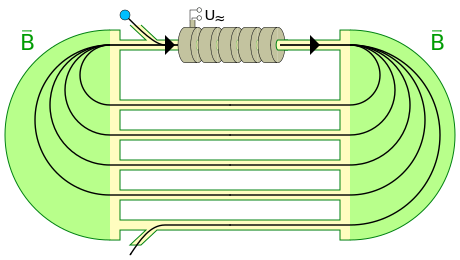
\includegraphics[width = 0.75\textwidth]{ExperimentalSetup/RacetrackMicrotronSketch.pdf}
\caption{Racetrack Microtron. The particles are sent to the linac, and the two deflection magnets make the particles recirculate, until the momenta exceed the capability of the magnetic field.}
\end{figure}

A racetrack microtron, as the one shown in the figure, is characterized by the energy gain per-cycle $\delta E$ given by the high-frequency electromagnetic field (HF). The energy gain is: 

\begin{align*}
\delta E \, = \, e U_{Linac} \cdot cos(\phi)
\end{align*} 

$U_{Linac}$ is the maximum voltage of the linac, and $\phi$ is the phase of the beam relative to the maximum of HF. Because the particle are accelerated by the linac, the beam consist in individual packets (bunches) whose rate correspond to the $\omega$ of HF. In order for the electrons to be accelerated for each recirculation step, they must arrive at the beginning of the linac with the correct phase $\phi$. For this it is important that the flight-time per cycle must be an integer or a multiple of the HF period.

\begin{equation} \label{eq:frequency}
f = \frac{1}{2 \pi} \cdot \dfrac{q}{\gamma m_{0}} \cdot B
\end{equation}
From this overview two conclusion can be drawn:
\begin{itemize}
\item To accelerate slow electrons, with $\gamma = (1,10)$, a magnetic field of $\SI{0.1}{\tesla}$ is used, in order to work with frequencies of ($\SI{2}{\giga \hertz}$,$\SI{2}{\giga \hertz}$), that are easy to control. However with higher energies the bending radii is higher, with a small magnetic field.
\item For high energy electrons $\gamma > 10$, to reduce the size of the deflection magnets, it is useful to increase the Magnetic field up to $\SI{1}{\tesla}$ of more. This let to accelerate the electrons using the same technology for $f \simeq \SI{}{\giga \hertz}$.
\end{itemize}

These conclusions justify the structure of MAMI: a cascade of microtrons to reach each time higher energies with the same acceleration frequency at each stage. \medskip
MAMI is composed by a sequence of 4 different microtrons, to achieve energies of $\SI{1.6}{\giga \electronvolt}$. The first stage, shown in figure \ref{fig:Accelerator}, is composed by two small microtrons. The first microtron RTM1 accelerate the particle to $\SI{14}{\mega \electronvolt}$ in 18 revolutions. The electrons are then sent to the second microtron that can accelerate the particle up to $\SI{180}{\mega \electronvolt}$. After passing the first stage, the beam is sent to the RTM3 (race track microtron 3), a large microtron with an end point energy of $\SI{855}{\mega \electronvolt}$. These 3 microtrons forms MAMI-B, which started operation in 1990-91. A fourth stage, MAMI-C, was built and started operation in 2007. This fourth stage is made by 4 bending magnets, with a bending angle of $90^{\circ}$, and it is designed to achieve energies of $\SI{1.6}{\giga \electronvolt}$. The design is different from the other race-track microtrons, and will not be explained, as it is not necessary for the experiment to reach such high energies.

\begin{figure}[hbtp]
\centering
\includegraphics[width=0.75\textwidth]{ExperimentalSetup/Racetrack.pdf}
\caption{Picture of the Racetrack RTM3 in MAMI-B. The Green square at the bottom is one of the deflector magnets, the other one is below the point where the photo was taken. The linac stage is on the left. The tubes at the center of the figure are the paths that the particle cross during the recirculation. The further away from the linac the greater the energy.}
\end{figure}

The operation principles of a microtron are simple to be described. First we conside the gyro-radius for relativist electrons, that is:

\begin{equation}
\qquad r = \dfrac{E \beta}{qcB}
\end{equation}

To have a coherent conditions, we must have that the flight-time $\tau = \frac{\lambda}{c}$ of the first recirculation must be an integer multiple of the HF, see equation \ref{eq:frequency}. This means that:

\begin{align*}
\lambda = \tau c =\dfrac{ 2 \pi c R }{\beta c} = \dfrac{2 \pi E}{q B} = m \lambda_{HF}
\end{align*}

For the other recirculation, we must have that the flight-time at energies $E_{i} = E_{n-1} + \delta E$ must be increased by an integer multiple of HF, too. This lead to the second equation:

\begin{align*}
\dfrac{2 \pi \delta E}{q B} = n \lambda_{HF}
\end{align*}

The minimum gain per cycle is then determined only by the strength of the magnetic field and wavelength $\lambda_{HF}$. These two equations together controls the dynamic of the race-track microtrons,

\subsection{Polarized Beam}
\commento{Here a subsection to explain how the polarized electrons are produced. Important to mention the systematic error for the polarization measurement (in our beam time we couldn't measure with Moller polarimeter, so this discussion is important for future experiment, however it's important to say something about it). Remember to explain how the spin are rotated to the transverse plane, and the $\frac{\lambda}{2}$} \medskip

For the beam-normal single spin asymmetry a vertical polarized beam is necessary. At the MAMI electron accelerator is possible to produce a vertical polarized beam with energy in the range $\SI{180}{\mega \electronvolt} - \SI{855}{\mega \electronvolt}$ \cite{Schlimme:2016rrp}. In this section the procedure to orient the beam vertically is presented, following an explanation of how the degree of polarization is measured. \medskip

The electron source used at MAMI is made by a strained GaAs/GaAsP super-lattice photo-cathode illuminated by circular polarized light. To alternate the sign of the light polarization, a fast Pockels cell ( \cite{}) is installed in the optical system of the electron source. The Pockels cell is a wave plate controlled by the electric field, that changes the helicity of the photons impinging on the electrons. A Pockels cell exploits the Pockels effect, that affects crystal with particular characteristics (lack of inversion symmetry). For this type of materials the refractive index is linearly dependent on the applied electric field. By controlling the refractive index with the electric field, the polarization state of the incident light beam is altered.
Once an photons imping on and electron, the extracted electron carries the same helicity of the incoming photon:
\begin{center}
\begin{equation}
\feynmandiagram [scale = 0.8, transform shape][baseline = (g)]{
	a [particle = \(e^{-}\)] -- [fermion] b  -- [fermion] c [particle = \(e^{-}\)],
	b -- [boson] d [particle = \(\gamma\)],};
\hspace{2cm}
(Jz)_{\gamma} = \pm 1 \qquad (Jz)_{e^{-}} = \mp \frac{1}{2} \rightarrow \pm \frac{1}{2}
\end{equation}
\end{center}

With the fast change of the Pockels cell it is possible to alternately revert the sign of the polarization. By the insertion of a $\lambda/2$ plate between the laser system and the photo-cathode the global polarization orientation of the electron beam can be reversed. This is particularly useful because this directly change the sign of the physical asymmetry measured by the detectors, and allows to identify systematic errors. This is useful done for longer beam time, where two sets of data are taken, reversing the orientation of the $\lambda/2$  wave plate. By comparing the results for the two sets of data, the influence of the optical system on the asymmetry measurement is estimated and can be corrected in the end result of the asymmetry. During the beam time of interest for this thesis, the $\lambda/2$ wave plate orientation was fixed. During previous beam time (\cite{Esser:2018vdp}). The beam polarization achieved with this source is roughly $P = 80 \% $, so the measured asymmetry are:

\begin{align*}
A_{measured} = P \cdot A_{n}
\end{align*}

The polarizations of the electrons just extracted from the source is still longitudinal. The Magnetic field is needed in order to rotate $\vec{P}$ from longitudinal polarization to transverse. For this purpose two devices are used: the \textbf{Wien filter} and a \textbf{double solenoid} located in the injection beam line, close to the the optical source: 

\begin{figure}[hbtp]
\centering
\includegraphics[width = \textwidth]{ExperimentalSetup/injection.png}
\caption{Beam line projection. This figure is taken from the paper \cite{Schlimme:2016rrp}}
\end{figure}

Following the picture, the spin of the electrons from the source are rotated first in the XY plane with a $90^{\circ}$ rotation, then the subsequent double solenoid align the spin to the vertical direction with another $90^{\circ}$ rotation. 
Once the beam passes the double solenoid, the electrons go through the linac, the microtron and in the end to the experimental hall, where the target of the experiments is installed. During the acceleration stage, the spin follows the precession motion due to the various magnetic fields of the accelerator, the precession, for a relativistic particle, is determined by the BMT equation.
However it is not necessary, due to our particular experimental setup, the BMT equation is quite simple: the magnetic field of the various bending magnets that constitute the microtron-cascade are always parallel to the vertical direction, because of this the cross product $\vec{B} \times \vec{P} = 0$, and the polarization remain constant. Only the residual horizontal component precedes during the motion. For conventional experiment that involve longitudinal polarization, after the first spin rotation due to Wien filter and the bending magnets close to the electrons source, there is a further rotation to be considered, due to the motion of the particle during the acceleration and recirculation in the microtron. Because of this, the rotation made by the Wien is set in such a way that after the second rotation due to the motion in the accelerator, the polarization has the correct alignment in the experimental hall. The rotation angles of the polarization vector through the accelerator are known from simulations and are also directly measured for relevant energies, for a beam of $\SI{570}{\mega \electronvolt}$ the rotation angle is $\ang{55}$ with an accuracy of $\pm \ang{2}$. In our case, this further rotation has only a small effect to the residual horizontal component, whose effect is negligible because it is accurately minimized by MAMI operators at the beginning of the beam time. Besides this, the effect of a small horizontal polarization on the asymmetry is small, knowing that typically the transverse asymmetries are one order higher that the $PV$.
At the beginning MAMI was not developed for experiment with transverse polarization. So it's not possible to measure directly the transverse component. However combining the measurement in the $XY$ plane, with the existing setup, it is possible to get the polarization value also in that direction. For this purpose a Moller, Comport and Mott polarimeters are used.


\subsection{Polarization Measurement}

To Measure the polarization of an electron beam different polarimeters can be used. Here we explain briefly the physics underlying the \textit{Mott} polarimeter, used in the experiment.
Consider an electron beam that is sent towards a nucleus of charge $Ze$. We know from theory \cite{MottElectron} that the spin of the incident electron interacts with the electromagnetic field produced by the nucleus.
The magnetic field seen by a particle with speed $\vec{v}$ near a nucleus is:

\begin{align*}
\vec{B}_{nucleus} = \frac{-\vec{v} \times \vec{E}_{nucleus}}{c}  = \frac{Ze}{mc r^{3}} \vec{L} 
\end{align*}

This magnetic field is coupled with the magnetic momenta of the electron $\mu_{e}$.

\begin{equation}
V = - \mu \cdot B_{nucleus} = \frac{Ze}{mcr^{3}} \vec{L} \cdot \vec{S}_{e^{-}}
\end{equation}

The second equation represents the spin-orbit interaction potential. This term yields the polarization dependence of the cross section, and it is exploited to obtain the polarization of the incident particles. Indeed the cross section can be modeled highlighting the dependencies on the spin $\vec{S}$:

\begin{align*}
\sigma(\theta) = I(\theta) [1 + S(\theta) \vec{P} \cdot \vec{n} ]
\end{align*}

Let's consider an incident particle that scatters from a nucleus at an angle $\theta$, as shown in the figure:

\begin{figure}[hbtp]
\centering
\includegraphics[width = 0.45\textwidth]{ExperimentalSetup/mottFig.png}
\caption{Scheme of the Mott scattering, the polarization is ortogonal to the plane,  $ \vec{n} = \frac{\vec{k} \times \vec{k'}}{|\vec{k} \times \vec{k'}|}$}
\end{figure}

The direction of $\vec{n}$ depends on whether scattering to the left or right is being considered. Let's suppose our initial beam has a polarization $P$, and so we compute the asymmetry $A(\theta)$ of the scattered electrons between left ($N_{L}$) and right ($N_{R}$). $N_{L}$ and right $N_{R}$ will be proportional respectively:


\begin{align*}
N_{L} &= N_{\downarrow}[1 + S(\theta)] + N_{\uparrow}[1 - S(\theta)] \\
N_{R} &= N_{\uparrow}[1 + S(\theta)] + N_{\downarrow}[1 - S(\theta)]  \\
A(\theta) = \frac{N_{L} - N_{R}}{N_{L} + N_{R}} &= \dfrac{N_{\downarrow}(1 + S(\theta)) + N_{\uparrow}(1 - S(\theta)) - N_{\uparrow}(1 + S(\theta)) + N_{\downarrow}(1 - S(\theta))}{N_{L} + N_{R}} = ... = P \cdot S(\theta)
\end{align*}


From the last equation we have a relation which give the beam polarization in terms of $A(\theta)$ (which is what is measured) and the asymmetry function $S(\theta)$ (known also as Sherman function). There are several calculation of the Sherman function, which is well-known for high energy electron scattering.

The total beam polarization is measured by a Moller polarimeter, in the experimental hall, with the beam polarization oriented longitudinally in the experimental hall. The Moller polarimeter can measure the longitudinal polarization of the beam.The other two polarimeters, Compton and Mott, located behind the injector linear accelerator (ILAC), are sensitive to the longitudinal and the trasverse horizontal components of the beam (with an energy around $\SI{3.5}{\mega \electronvolt}$ at this stage). The procedure for the allignment is the following: at the beginning of the beam time the Mott polarimeter is used for different settings of the solenoidal field, with the Wien filter angle equal (nominal) to $\ang{90}$. The aim is to minimize the horizonal polarization component after the rotation performed by the double solenoid, changing the solenoidal magnetic field. Then a second optimization follows, using the Moller polarimeter for different Wien filter angles is performed. With the new Wien filter settings, another measurement is performed with the Mott polarimeter.

\subsection{Moller and Compton polarimeters}


\section{Experimental Hall Setup}

\commento{Describing the A1 room, how the spectrometers are operating (+ figures), a picture of the target and the important parameters, like thickness. Also mention the convention to use target with$10 \%$ of the radiation length, to avoid double scattering.  Mention that we need the Wobbler magnet to change the hitting position of the beam to prevent the target from melting. Here it's important to mention that the electron are deflected on the vertical direction, because of the high beam intensity
Then add a picture of the beam-line.}

Until now we have described how MAMI produce to accelerate the electrons, however we have not presented the structure where the beam is delivered and various experiments are carried out. \\
Actually MAMI has 2 different hall, named with the capital letter A followed with a number, which indicate also the different collaboration that work with the experiments. In A2, as an example, photo-nuclear reactions are studied to investigate the fundamental physics at the scale of nuclear dimensions. The experimental hall where the experiment treated described in this thesis is conducted is the A1 hall. We will describe briefly the main operating detectors that are installed and the details that are interesting for the \transv    measurement. \bigskip

\begin{figure}[hbtp]
\centering
\includegraphics[width = 0.6\textwidth]{ExperimentalSetup/Accelerator.pdf}
\caption{Scheme of the accelerator, with the different experimental halls. A third hall previously used for the A4 experiment, measuring the strange quark content of the proton, is now being used for the novel MESA accelerator and its experiments.}
\label{fig:Accelerator}
\end{figure}

In A1, experiment with fixed targets are conducted. The electrons can be delivered with an energy up to $\SI{1.6}{\giga \electronvolt}$, after passing the last acceleration stage (HDSM, in the figure). Because the electron energy of our experiment is $\SI{570}{\mega \electronvolt}$, the beam will pass through the first acceleration steps, the linac (linear accelerator) and Race-track system and when the desired energy is achieved the electrons will be sent to the A1 experimental hall. 

\newpage
\begin{figure}[hbtp]
\centering
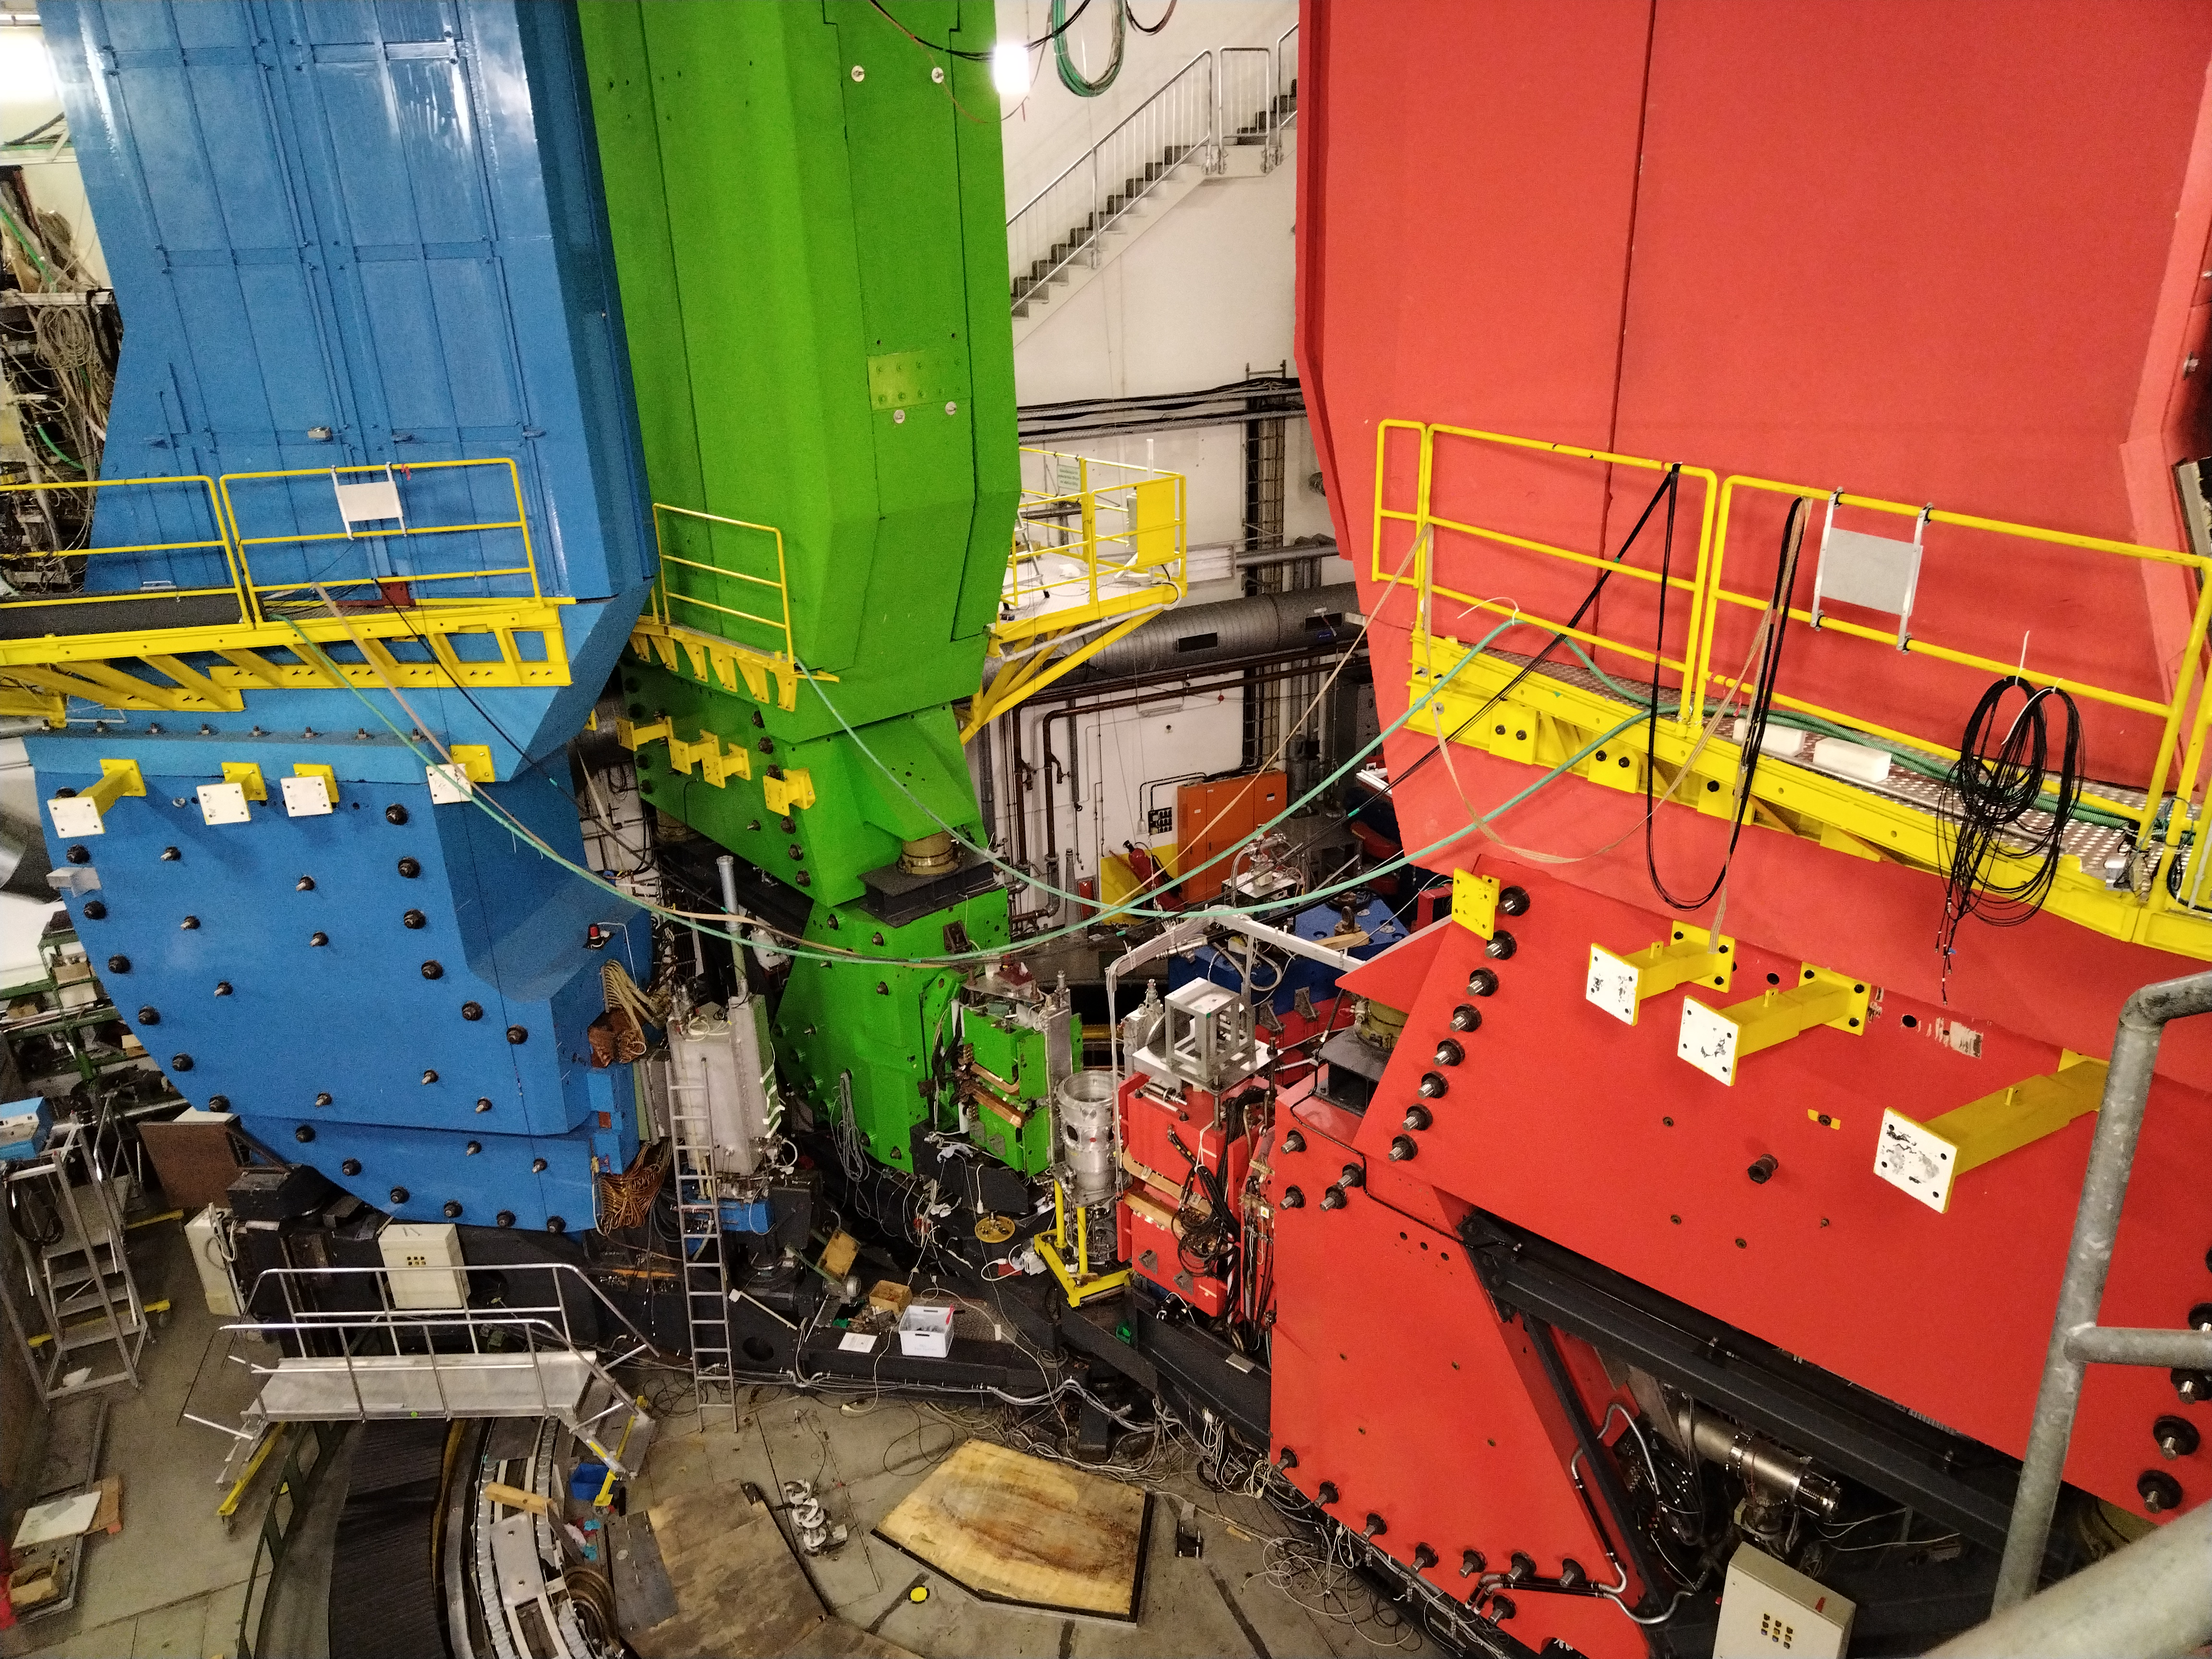
\includegraphics[width = \textwidth]{figures/twoSpektrometer.pdf}
\caption{Picture of the A1 spectrometers hall, the spectrometers red and blue are used during this experiment. At the center of the picture is possible to observe the scattering chamber.}
\end{figure}

Inside A1 hall three large magnetic spectrometers are placed on a circular rail-track around the target chamber. These spectrometers where designed and built in $1993$ to perform high precision measurement of electron scattering in coincidence with other hadron detection, with an high resolution in the determination of the particle momenta $\frac{\delta p}{p} < 10^{-4}$. The spectrometers develop vertically with an height of $\SI{15}{\meter}$, for this reason the scattered electrons and the other particles are deflected with the use of the magnetic field respect to the scattering plane. The following figure shows the path the particle scattered from the target:
\begin{SCfigure}[30][ht]
\centering
\caption{Image of the spectrometers of A1 hall. The spectrometers can be rotated using a system of rail-tracks that are visible at the bottom of the image. The electrons are scattered and then deflected in the vertical direction by the magnetic field (green lines). This picture is taken from behind the target. The target is roughly at the center of the image where the two green lines join. The electron are coming from the opposite direction, respect with the spectrometers.}\label{fig:TwoDetectors}
\includegraphics[width = 0.45\textwidth]{ExperimentalSetup/A1_Dietro.pdf}
\end{SCfigure}
The spectrometers used for the transverse asymmetry are the ones shown in the picture. There are multiple reasons why the particle are deflected on the vertical direction, we summarized them in two points: 
\begin{itemize}
\item reason of space, due to the fact the an horizontal setup would not fit with the dimension of the building in addiction to the fact that this would not allow to rotate the spectrometers by a variety of angles that the vertical orientation does
\item reduce background and noise, in fact the high beam intensity that is possible to reach at MAMI is a source of noise and background event which can be cut off detecting the particle far from the interaction point.
\end{itemize}      
Once a particle is scattered in the acceptance region of the spectrometers, it is deflected by the magnetic field and passes through the drift chamber, which occupies the first third in height of the spectrometers. 
When the particle is at the height of the platform in the figure \ref{fig:TwoDetectors}, it impinges on a layer of plastic scintillator, and after that a Cherenkov detector which measures the particle speed $\vec{v}$.We have a picture \ref{fig:internal} of the spectrometers internal, taken during the installation of the two detectors.The determination of both the particle speed $\vec{v}$ and momenta (drift chamber) allows to identify the particles. Despite the possibilities offered by the already existing setup, for the beam time of interest none of these components was used directly in the estimation of $A_{n}$. The reason is due to the high intensity of the beam that is used in the experiment, which is far from the optimal operating conditions of the components, that are suited for rates lower than the ones expected for beam normal single spin measurements. The spectrometers are used indirectly for the alignment of scattered electrons to the focal plane of our detectors.
\newline
\begin{figure}[!hbtp]
\centering
\includegraphics[width=0.4\textwidth]{ExperimentalSetup/Detectors/position.pdf}
\caption{Internal of the spectrometer. This image was taken during the installation of the detector A inside the red spectrometer, that is accessible from the platforms visible in the picture \ref{fig:TwoDetectors}}
\label{fig:internal}
\end{figure}
\newpage
\section{Detector Description} \label{detectors}
In this section we will describe the electronics and the detectors used to measure the \transv .
For this experiment we are going to measure the \transv at one fixed angle, corresponding to a transferred momentum of $Q = \SI{0.2}{\giga \electronvolt}$. The electrons detection is 
made via two thin blocks of fused-silica that are coupled to PMTs. When a scattered electron hits the fused-silica (refractive index $n = 1.45$) Cherenkov light is emitted. The emitted Cherenkov light can interact with the electrons of the material, which, in turn, can hits the PMT dynode. This sequence of event triggers the PMT and produce an output signal.

In the experiment two detectors are installed and read-out independently. The detector A is placed at an angle of $+\theta$, while detector B is placed at $-\theta$. We expect to measure the same absolute value of the transverse asymmetry, with an opposite sign due to the different orientation. 
The two detector are made by 3 PMTs and 8 PMTs coupled with two blocks of fused-silica, a scheme of the detector is shown below:

\begin{figure}[hbtp]
\centering
\subfloat[][\emph{Detector B scheme.}]{
\includegraphics[width = 0.40\textwidth ]{ExperimentalSetup/Detectors/DetectorB.pdf}}
\subfloat[][\emph{Detector A scheme.}]{
\includegraphics[width = 0.55\textwidth ]{ExperimentalSetup/Detectors/detectorA.pdf}}
\end{figure}

These two detectors are placed inside the spectrometers presented in \commento{aggiungere referenza}, between the top of the drift-chamber, which occupies the first third in height of the spectrometer, and just below a panel of scintillator. During the experiment, the drift chamber of the spectrometers is turn off, and also the PMTs coupled to the spectrometer scintillators are not powered.
As we mention above, the scattered electron are deflected in the vertical direction by the magnetic field of the spectrometer. 
At this moment, it is important to mention the differences between the new and the old electronic setup. In the old electronic setup the output signal of the PMTs was integrated during the time interval of each sub-event, and therefore the single scattered electron could not be counted. The advantage of this method is that the electronics is more simple. However, this old method is affected by a baseline noise and it is not good for the future experiments with lead target, where the expected rates are lower than the rates on carbon.
With the new electronics, all the single electrons are counted, and this will allow the future measurements with lead, improving the accuracy. 

\begin{figure}[hbtp]
\centering
\subfloat[][\emph{Detector B}]
	{\includegraphics[width = 0.35\textwidth]{figures/504px-Blackfalcon.jpg}} \quad
\subfloat[][\emph{Detector A}]
	{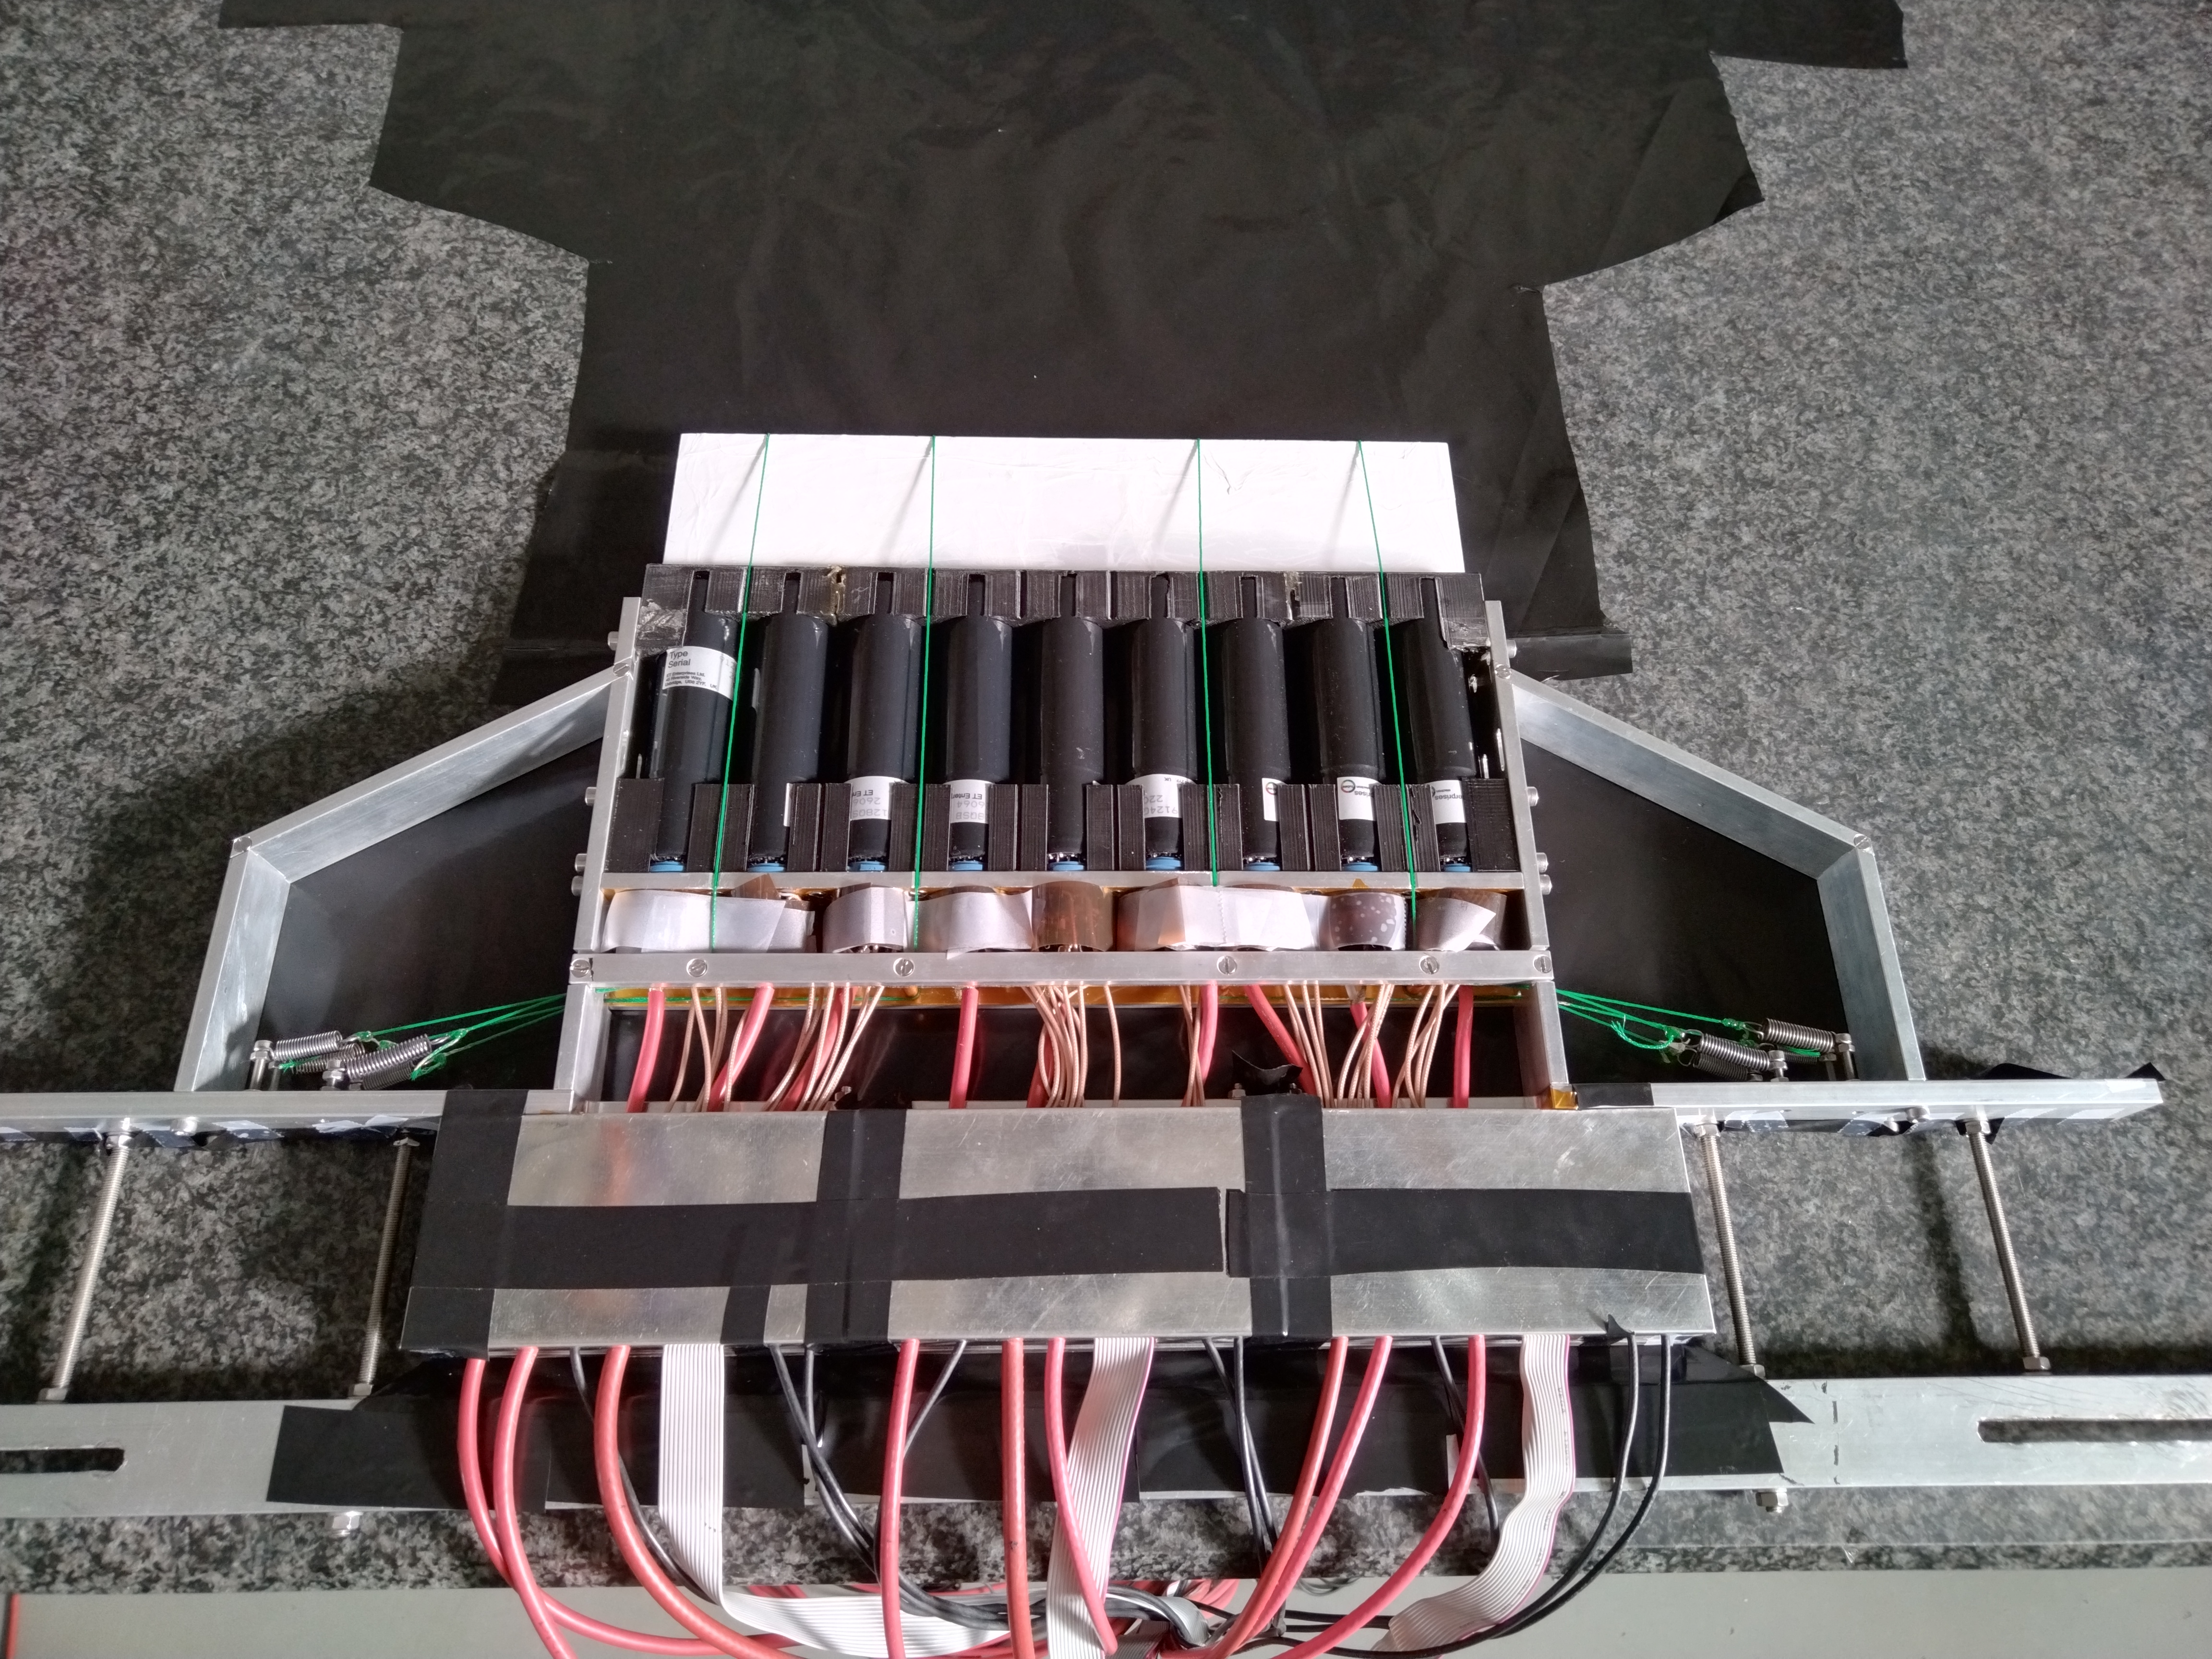
\includegraphics[width = 0.45\textwidth]{figures/IMG_20221110_122246.pdf}} \quad
	\label{fig:Detectors}
\caption{Picture of the two detector taken in the clean room. The white blocks are the fused silica that produces the Cherenkov light, the cylinders below are the PMTs.}
\end{figure}

Here we report the characteristic of the two detector that are relevant for the data analysis: 

\begin{itemize}
\item detector B size: $\SI{7}{\centi \meter} \times \SI{10}{\centi \meter} \times \SI{1}{\centi \meter}$
\item detector A size: $\SI{7}{\centi \meter} \times \SI{30}{\centi \meter} \times \SI{1}{\centi \meter}$
\item Number of dynodes: 12
\item The Power voltage for the PMT in negative, in the range of ($\SI{-900}{\volt}$, $\SI{-1100}{\volt}$)
\item refraction index $n$ of the fused-silica is $1.45$.
\end{itemize}


\section{Beam Monitors}
\commento{Explain how the monitors for the beam parameters work. (this section could be long, however the way these parameters are measured is particular, so it is important to explain everything properly).}

In MAMI, several monitors are placed along the beam line in order to to check beam quality and measure parameters such as current intensity, energy and relative position of the beam. This section summarizes an explanation of the operating principles of the monitors installed at MAMI. The explanation will be partial, some details will be given in the appendix, however for a complete discussion please refer to the following paper (\cite{M_Dehn}).

The monitors available at MAMI are quite specific for the standard of the particle accelerators. Resonant cavities are used to measure the various quantities, with the underlying physical principle that the passage of charged particles through these cavities can excitate some electromagnetic resonant modes\footnote{TM mode, where the magnetic field is completely trasverse respect to particle momenta} which can be detected and analyzed by an analog circuit to measure the beam parameters.
Before going into the details, is necessary to define some quantities that will be used later in the explanation. We define $r_{s}$, the Shunt-impedance as :

\begin{equation}
r_{s} = \frac{|V_{\|}|^{2}}{P}
\end{equation}

$P$ is the power absorbed by the cavity when a particle excites one of the resonant mode, instead $V_{\|}$ is defined as the effective voltage surpassed by a charged particle along a straight line, which can be computed as:

\begin{align*}
V_{\|} = \frac{1}{q}  \int_{s_{0}}^{s^{1}} \vec{E}_{s} \vec{e_{s}} \,ds
\end{align*}

The Shunt impedance is a measure of the interaction strength between a cavity and a charged particle, and can be expressed also in another way, introducing the $Q$ value of the cavity, $W$ the maximum energy stored and $f_{r}$ the frequency of resonance:

\begin{align*}
r_{s} = \dfrac{|V_{\|}|^{2} Q}{2 \pi f_{r} W}
\end{align*}

When the beam travels through the cavity, the particles release energy that excites the  mode. The power $P_{HF}$ extracted from the beam is related to the beam current: 

\begin{align*}
P = \iota^{2} r_{s}
\end{align*}

An antenna is used to decouple part of the energy from the cavity and send it to a circuit which produces an analog output signal. Indicating with $\kappa$ the coupling constant of the antenna, the previous relation needs to be modified introducing a new factor $ \frac{\kappa}{(1 + \kappa)^2}$. In a Cylindrical resonator, the same type installed at MAMI, the resonance frequency of the different oscillascion modes is expressed by the formula 

\begin{align*}
f_{m,n,p} = \frac{c}{2\pi \sqrt{\epsilon_{r} \mu_{r}}} \sqrt{(\frac{x_{m,n}}{R})^{2} + (\frac{p \pi}{L})^{2}}
\end{align*}

The constant in the formula are:

\begin{itemize}
\item $c$ is the light speed.
\item $\epsilon_{r}, \mu_{r}$ are the magnetic and dielectric costant of the material.
\item $x_{m,n}$ it the n-th zero of the m-th Bessel function.
\item $R$ and $L$ are the radius of the cylindrical cavity and his lenght.
\item \commento{$p$ I dont' know yet.}
\end{itemize}

This formula can be obtained solving the Maxwell equations with cylindrical boundary condition, the eigenvalues are then given by the formula above. \\
If the frequency of the Beam bunch is equal to the resonant frequency $f_{m,n,p}$ of the cavity, a TM mode is excited. At MAMI high quality monitors are installed, quantitatively all the monitors have a $Q \simeq 10000$, that means that $\frac{\nu}{\delta \nu} \simeq 10000$. This means that the frequency of the beam buch must be very close to the frequency of the resonant cavity. At MAMI the frequency used for all the resonators is $\SI{2.449532}{\giga \hertz}$ or a multiple of it. The beam bunch frequency is the same, and it is controlled by the MAMI-master oscillation signal, that is the reference signal for all the MAMI monitors.

\begin{figure}[hbtp]
\centering
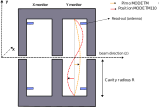
\includegraphics[width = 0.6 \textwidth]{ExperimentalSetup/Monitors.pdf}
\caption{Scheme of the Cylindrical cavities installed at MAMI. In red we have the $TM_{110}$ mode, used to measure the position of the beam, in yellow the $TM_{010}$ mode, to measure the intensity of the beam.}
\end{figure}

Depending on the $TM$ mode excited, we have a different signal in the cavity, so a different signal collected by the antenna. The relevant quantity that is detected is the power $P_{HF}$ absorbed by the antenna. For the $TM_{010}$ mode, the power is 

\begin{equation}
P_{HF} = i^{2} r_{010} \frac{\kappa}{(1 + \kappa)^{2}}
\end{equation}

The power absorbed by the antenna is directly dependent on the beam current. Because the rage values are typically in the range of $\SI{}{\pico \watt}$ to $\SI{}{\milli \watt }$, the signal is processed in close proximity of the installed monitors. In the signal process, the input signal of the antenna in coupled to the master-oscillation signal, so the output signal is given by the formula:

\begin{equation}
U = \sqrt{P_{HF}} \cos(\phi - \phi_{LO})
\end{equation}

the phase $\phi$ is the phase of the resonant mode or the phase of the beam bunch, while the phase $\phi_{LO}$ is the phase respect to the master-oscillation signal, and can be adjusted by a phase shifter of the circuit. The output voltage signal can be read out with the oscilloscope or digitalized and saved with other devices. To measure the beam intensity is important to minimize $\phi - \phi_{LO}$, to maximize the signal amplitude, and then the output signal is ready to be analyzed.

\begin{figure}[hbtp]
\centering
\includegraphics[width = 0.5\textwidth]{ExperimentalSetup/PIMOphase.pdf}
\caption{Plot of the phase $\phi$ versus the output signal. The phase optimization was done selecting the working point in correspondence of the peak.}
\end{figure}

The measurement of the $x,y$ position follows in principle the same procedure. In this case the $TM_{110}$ is acquired. The reason is clear, because it is possible to calculate that for this mode the $r_{shunt}$ is proportional to the beam position on the $x,y$ plane. So The power absorbed by the antenna can be written:

\begin{equation}
P_{HF} = i^{2} r_{110} \frac{\kappa}{(1 + \kappa)^{2}} K x^{2}
\end{equation} 
 
The output signal, that is read by our setup, is proportional to the square root of the absorbed power:

\begin{equation}
\sqrt(P_{HF}) = costant \cdot U \, \cdot \, i   \cdot x
\end{equation} 

The beam parameter are then given inverting the above formula 

\begin{equation} \label{eq:SignalToVfc}
x \simeq \frac{\sqrt(P_{HF})}{i}
\end{equation}

Where the exact conversion coefficients are not known, and are determined during the calibration phase, at the beginning of the beam time.
To measure the beam energy, a different approach is used. In principal, the energy monitor (ENMO) consist of 2 cavities in the RTM3. One is located in the last recirculation pipe, the other one on the part of the beam line, where the acceleration takes place.
The two monitors are synchronized to the master oscillation and measure the phase of the bunches of electrons. When during their travel from the first cavity to the second cavity, the beam passes through the magnet and does one half turn. Now, if the energy is slightly larger, the radius of the turn will be slightly longer. This means that there is an extra time between the two bunches, that can be measured as a small phase shift in the $\SI{570}{\mega \electronvolt}$ recirculation. From this it is possible to obtain a value for the difference of energy to the nominal energy.

\subsection{Beam stabilization}

The beam stabilization is an essential component of the experiment. The values of $A_{n}$ that we want to measure are in the order of ten $ppm$, so it is important to reduce other contributions that can be related to variations in the beam parameters. 

\section{Electronics}
\commento{Short introduction about the old electronics setup and why a new versions is needed, then describe all the electronics used for our experiment:
\begin{itemize}
\item Nino board for collecting the data from the PMTs
\item VFCs for collecting the data from X21,X25,Y21,Y25,ENMO,I21,I13
\item master board for collecting the monitors data/controlling the source/wobbler magnets.
\item small boxes for switching from new electronic read-out to the old electronics read-out (spectrometers DAQ)
\end{itemize}}


\subsection{VFCs}

Some parameters which describe the beam are needed in order to take into account possible effect in the measure of the transverse asymmetry. The relevant data are the position in the $(x,y)$ plane, the incident angles on the target, the current and energy of the beam. All this values are collected using the already existing monitors. \\
To collect the data from the monitors, single and multichannel, synchronous voltage-to-frequency converters (AD7742) are used. This devices contain an analog modulator that is able to convert the input voltage into an output pulse train, whose frequency is proportional to the input voltage. 

\begin{wrapfloat}{figure}{I}{0pt}
\includegraphics[width=0.5\textwidth]{ExperimentalSetup/Vfc.pdf}
\caption{Frequency versus Voltage}
\vspace{10pt}
\end{wrapfloat}

The VFCs are powered with an external voltage of $\SI{5}{\volt}$. They measure an input voltage in the range of ($-V_{ref}$, $V_{ref}$). An external clock signal, with a frequency $F_{CLKIN} = \SI{5.88}{\mega \hertz}$ is created externally and synchronous to the gate-length.
The analog input signal is sampled with by a switched capacitor, with a rate that is equal to $F_{CLKIN}$.
The comparator produces a number pulses; the frequency of the output signal is proportional to the input voltage, with $-V_{ref}$ equal to $0.5 \% \cdot f_{CLKIN}$ and $+V_{ref}$ equal to $0.45 \% \cdot f_{CLKIN}$ \cite{VfcDatasheet}, where the first correspond to $\SI{0.0}{ \volt}$ in input and the second to $V_{ref}$. The relation between the output frequency and the input voltage is the following:

\begin{equation}
V_{in} = V_{ref} (2 \frac{f_{out} - 5\% F_{CLKIN}}{40 \% \cdot F_{CLKIN}} -1)
\end{equation}

The data are acquired counting the number of pulses that come from the comparator, so we can substitute to $f$ the number of pulses (the two quantities are proportional), and we end with:

\begin{equation} \label{eq:Vfc}
V_{in} =  V_{ref}[2 \cdot \dfrac{N_{pulses} - 5 \% N_{CLKN}}{40 \% N_{CLKN}} - 1]
\end{equation}

\subsection{Nino Board} \label{NINO}

The NINO board is our data acquisition system for the PMT counts. It is made by $32$ analog input channels and it is powered with $\pm \SI{5}{\volt}$. Each channel has an attenuator, and the signal passes through that before going to the Comparator, which compares the signal to the threshold. The Output signal is a Low-voltage differential signal (LVDS). Each comparator can handle eight channels and for each of them it is possible to define a global threshold. With the current settings of NINO board, it is possible to change the threshold of each channel acting on another value, the attenuation, which decreases the value of the global threshold. Attenuation and threshold are set using 12 bit DACs, corresponding to interval of $(0 ; 4095)$. \medskip
The NINO board is designed in such a way that collects the Input charge of the signal, operating with a $\SI{30}{\pico \farad}$ capacitor. The output signal amplitude is proportional to the input charge, and it is sent to the discriminator. Our interest is only to count the number of scattered electron, so we do not intend to measure the input charge, but only a signal is produced or not.

\begin{figure}[hbtp]
\centering
\includegraphics[width = 0.75\textwidth]{ExperimentalSetup/NINO.pdf}
\caption{Nino Board}
\label{fig:NinoBoard}
\end{figure}

Two Nino board are used in the experiment, one for detector A and one for detector B. For the experiment discussed in this thesis, we will use only 8 channel for detector A and 3 channel for detector B, since this is the number of the input signals coming from the two detectors. For the future experiments more channel will be used, splitting the analog input signal in 4 different signal, sending it to 4 different input channel of the board. This is useful because changing individually the attenuation value, we can define 4 different thresholds for the same signal coming from a single PMT. This is useful to compare different values of threshold, for example to study how the noise affects the measurement, and see what is the right compromise between signal and noise  .
The way we selected the threshold is explained in the following chapter (Analysis).

\subsection{Master Board}

\begin{figure}[hbtp]

\centering
\includegraphics[width = \textwidth]{ExperimentalSetup/masterboard.pdf}
\caption{Scheme of the master-board, the device that coordinates all the electronics for the experiments, and send the data to the computer in the control room.}
\end{figure}


\chapter{Test and beam time analysis} \label{analysis}

\begin{outline}[enumerate]
\1 development of the analysis program.
\1 testing the analysis program with montecarlo data.
\1 Test of the detectors in the Lab.
\1 Beam line description.
\1 Data Analysis
	\2 thresholds scan
	\2 Rates on $Pb^{208}$.
	\2 Beam related asymmetry correction.
	\2 $C^{12}$ Asymmetry.
\end{outline}

\paragraph{Introduction}
In this chapter we discuss the electronic test that have been carried out in the laboratory, and the calibrations that need to be done
in order to calculate, from the raw data, the final data ready for the analysis.
The test in the lab consist in checking that the photomultipliers are working and that the electronics that take care of acquiring the data do not have any errors.
For the calibrations, since several beam parameters are needed for the analysis, it's importat to obtain the correct scaling factor to convert the Raw Data collected by the \textit{VFC}s to data with the right physical units, as the $X,Y$ impact point of the beam on the target, the beam energy $E$, the beam currer $I$ and the scattering angles $\theta_{x}$ and $\theta_{y}$.

\section{Data tree}
Explain how we compute all the values for the data tree, the position of the beam on the target, the angle, the correlated-difference values...

\section{Detectors test}

{\bfseries Explain the test of the two detectors in the lab, how we select the threshold, the correlation of the pmts and coincidence to select the threshold. Mention also that we observed two knees in the plot of counts vs. attenuation.}

The Nino board, which digitizes the signal from the PMTS, has two parameters which can be used to select the internal threshold of the discriminator, to cut the low amplitude signals and can be adjusted changing the settings of the DAQ program. These two parameters are \textit{Threshold} and \textit{Attenuation}. \textit{Threshold} means directly the charge value necessary for an impulse certain shape to be accepted by the signal discriminators. However the "physical" threshold can be also modified changing the \textit{attenuation}. The relation between threshold and attenuation is not linear, but follows:

\begin{figure}[hbtp]
\centering
\subfloat[][\emph{Threshold dependence against attenuation} \label{NinoDocu}]{
\includegraphics[scale=0.4]{Analysis/ThrvsAtt.png}}
\end{figure}

For our purposes, we select a common threshold values for all the pmts, and we decided to change only the attenuation values.\\
Before the Beam time, some test with the two detectors were performed, to check that the pmts were still working after some years of inactivity, and that the new electronic was able to count properly the pulses and store the data. For this studies, we didn't have a radioactive sources to employ, so we moved the two detectors in the workshop of the accelerator, and we use the cosmic rays rate as a probe. 

Knowing that the expected number of event for cosmic rays is about $1 \frac{event}{\SI{}{\centi \meter\squared} \SI{}{\second}}$ we can compute the expected values for the number of events. We decided to take 1 minute long acquisition for both the two detectors, this leads to $70$ expected events for detector B  and  $100$ events for detector A.  \smallskip

The first step is to select a good point of work for the threshold. So, fixing the value of the threshold parameter for the NINO board, we took several acquisitions, each of them one minute long, increasing each time the attenuation. We powered the pmts with a negative voltage around $ \SI{-1000}{\volt}$, as suggested in the datasheets, and covered the cherenkov detector with a shielding blanket, to avoid ambient light simulating a signal.

\begin{figure}[hbtp]
\centering
\subfloat[][\emph{Attenuation scan for Detector B}]{
\includegraphics[width = 0.45\textwidth]{Analysis/AttenuationB.pdf}}
\subfloat[][\emph{Detector B Counts versus attenuation,the area with constant counts is highlighted }]{
\includegraphics[width = 0.47 \textwidth]{Analysis/AttenuationBlinear.pdf} }
\end{figure}

We observed a small knee in the plot, around the zone of 580 − 600 of attenuation, where the number of counts was almost costant, roughly equal to the number of expected events from muons hitting the detector. Then we observe a big edge for attenuation = 1000. Looking at the plot \ref{NinoDocu}, we assume that the attenuation values are so high that electronic noise is no longer rejected, in fact the counts grow enormously. The attenuation was set at 600.

The next step was to study the statistical fluctuation of the counts, so we collected 10 acquisitions, each of them 1 min long. The measured values are reported in the table below:

\begin{center}
\begin{tabular}{|c|c|c|c|}
\hline 
Pmt: & 1 & 2 & 3 \\ 

1 & 58 & 60 & 62 \\ 
\hline 
2 & 62 & 55 & 59 \\ 
\hline 
3 & 61 & 59 & 70 \\ 
\hline 
4 & 73 & 66 & 70 \\ 
\hline 
5 & 68 & 66 & 56 \\ 
\hline 
6 & 59 & 52 & 64 \\ 
\hline 
7 & 69 & 74 & 77 \\ 
\hline 
8 & 48 & 49 & 57  \\ 
\hline 
9 & 70 & 54 & 58 \\ 
\hline 
10 & 60 & 61 & 66\\
\hline
\end{tabular} 
\end{center}

This data are interesting to check if the counts are following the theoretical distribution of the events expected for cosmic rays at sea level. If the pmt are working in a good mode, we know that the number of counts should be Poisson-distributed:

\begin{equation}
Pdf(\mu,k) =  \frac{\mu^{k}}{k!} e^{-\mu}
\end{equation}

The variance of the poisson distribution is equal to the mean of the counts, and we expect the same behaviour also for the sample mean and the sample variance:

\begin{align*}
\begin{split}
\mu_{1} = 62.8	\qquad \sigma^{2}_{1} = 54.40 \qquad r_{12} = 0.66\\
\mu_{2} = 59.6	\qquad \sigma^{2}_{2} = 57.15 \qquad r_{23} = 0.65\\
\mu_{3} = 63.9	\qquad \sigma^{2}_{3} = 46.98 \qquad r_{13} = 0.35 \\
\end{split}
\end{align*}

We report also the correlation $r_{xy}$ between the pmt. The result are fine: we are able to see a positive correlation between adjacent pmt, and as expected the correlation is lower in the case of the more distant. This is explained by the lower probability that the photons of Cherenkov radiation light up at the same time the more distant pmt.
We can test that the data follow a possion distribution using the well-known Gosset test, defined as:

\begin{equation}
\chi^{2}_{n-1} = \sum_{i = 1}^{n} \dfrac{(Oss_{i} - Att_{i})}{Att_{i}}
\end{equation}

We report the result obtain with the data for detector B, the test shows that there is good agreement with the hypothesis that the count are really poisson-distributed.

\begingroup
\setlength{\tabcolsep}{8pt} % Default value: 6pt
\renewcommand{\arraystretch}{1.2} % Default value: 1
\begin{center}
\begin{tabular}{|c|c|c|c|}
\hline 
Pmt: & 1 & 2 & 3 \\ 
\hline
$\chi^{2}_{9}$ & 8.52 & 8.45 & 6.37 \\ 
\hline
\end{tabular} 
\end{center}
\endgroup

To convince oneself that the pmt are actually measuring signals given by the passage of cosmic rays, and not noise, we exploit the possibility of we exploited the possibility of placing one pmt in coincidence with the others. If we are able to observe correlation between the counts, we can conclude that the detection electronics are working correctly. \\
One pmt was placed over the detector and we read out the counts simultaneously.

\begin{center}
\begin{tabular}{|c|c|c|c|c|}
\hline 
pmt & 0 & 1 & 2 & 4 (in coincidence) \\ 
\hline 
1 & 63 & 57 & 72 & 28 \\ 
\hline 
2 & 55 & 51 & 64 & 18 \\ 
\hline 
3 & 62 & 53 & 75 & 27 \\ 
\hline 
4 & 71 & 62 & 75 & 33 \\ 
\hline 
5 & 68 & 59 & 49 & 23 \\ 
\hline 
6 & 57 & 55 & 63 & 18 \\ 
\hline 
7 & 70 & 64 & 64 & 24 \\ 
\hline 
8 & 50 & 69 & 69 & 25 \\ 
\hline 
9 & 65 & 62 & 62 & 19 \\ 
\hline 
10 & 74 & 71 & 77 & 28 \\ 
\hline 
\end{tabular} 
\end{center} 

As above, we report the sample mean, the variance and the correlation between the pmt in coincidence and the detector B:

\begin{equation*}
\begin{split}
\mu_{0} = 63.5 \qquad \sigma^{2} = 58.9 \qquad r_{04} = 0.49 \\
\mu_{1} = 60.3 \qquad \sigma^{2} = 43.3 \qquad r_{14} = 0.38 \\
\mu_{2} = 67.0 \qquad \sigma^{2} = 71.1 \qquad r_{24} = 0.65 \\
\end{split}
\end{equation*}

We observe a positive correlation $r_{04},r_{14},r_{24}$ for the pmt in coincidence, this is a strong evidence that the signals are correlated and that some particles are hitting the fused silica sequentially. \smallskip

\begingroup
\setlength{\tabcolsep}{8pt} % Default value: 6pt
\renewcommand{\arraystretch}{1.2} % Default value: 1
\begin{center}
\begin{tabular}{|c|c|c|c|c|}
\hline 
Pmt: & 1 & 2 & 3 & pmt in coincidence \\ 
\hline
$\chi^{2}_{9}$ & 8.95 & 6.44 & 10.96 & 9.52\\ 
\hline
\end{tabular} 
\end{center}
\endgroup
\smallskip

We also check at the oscilloscope if we were able to observe three negative peaks at the same time: 

\begin{figure}
\centering
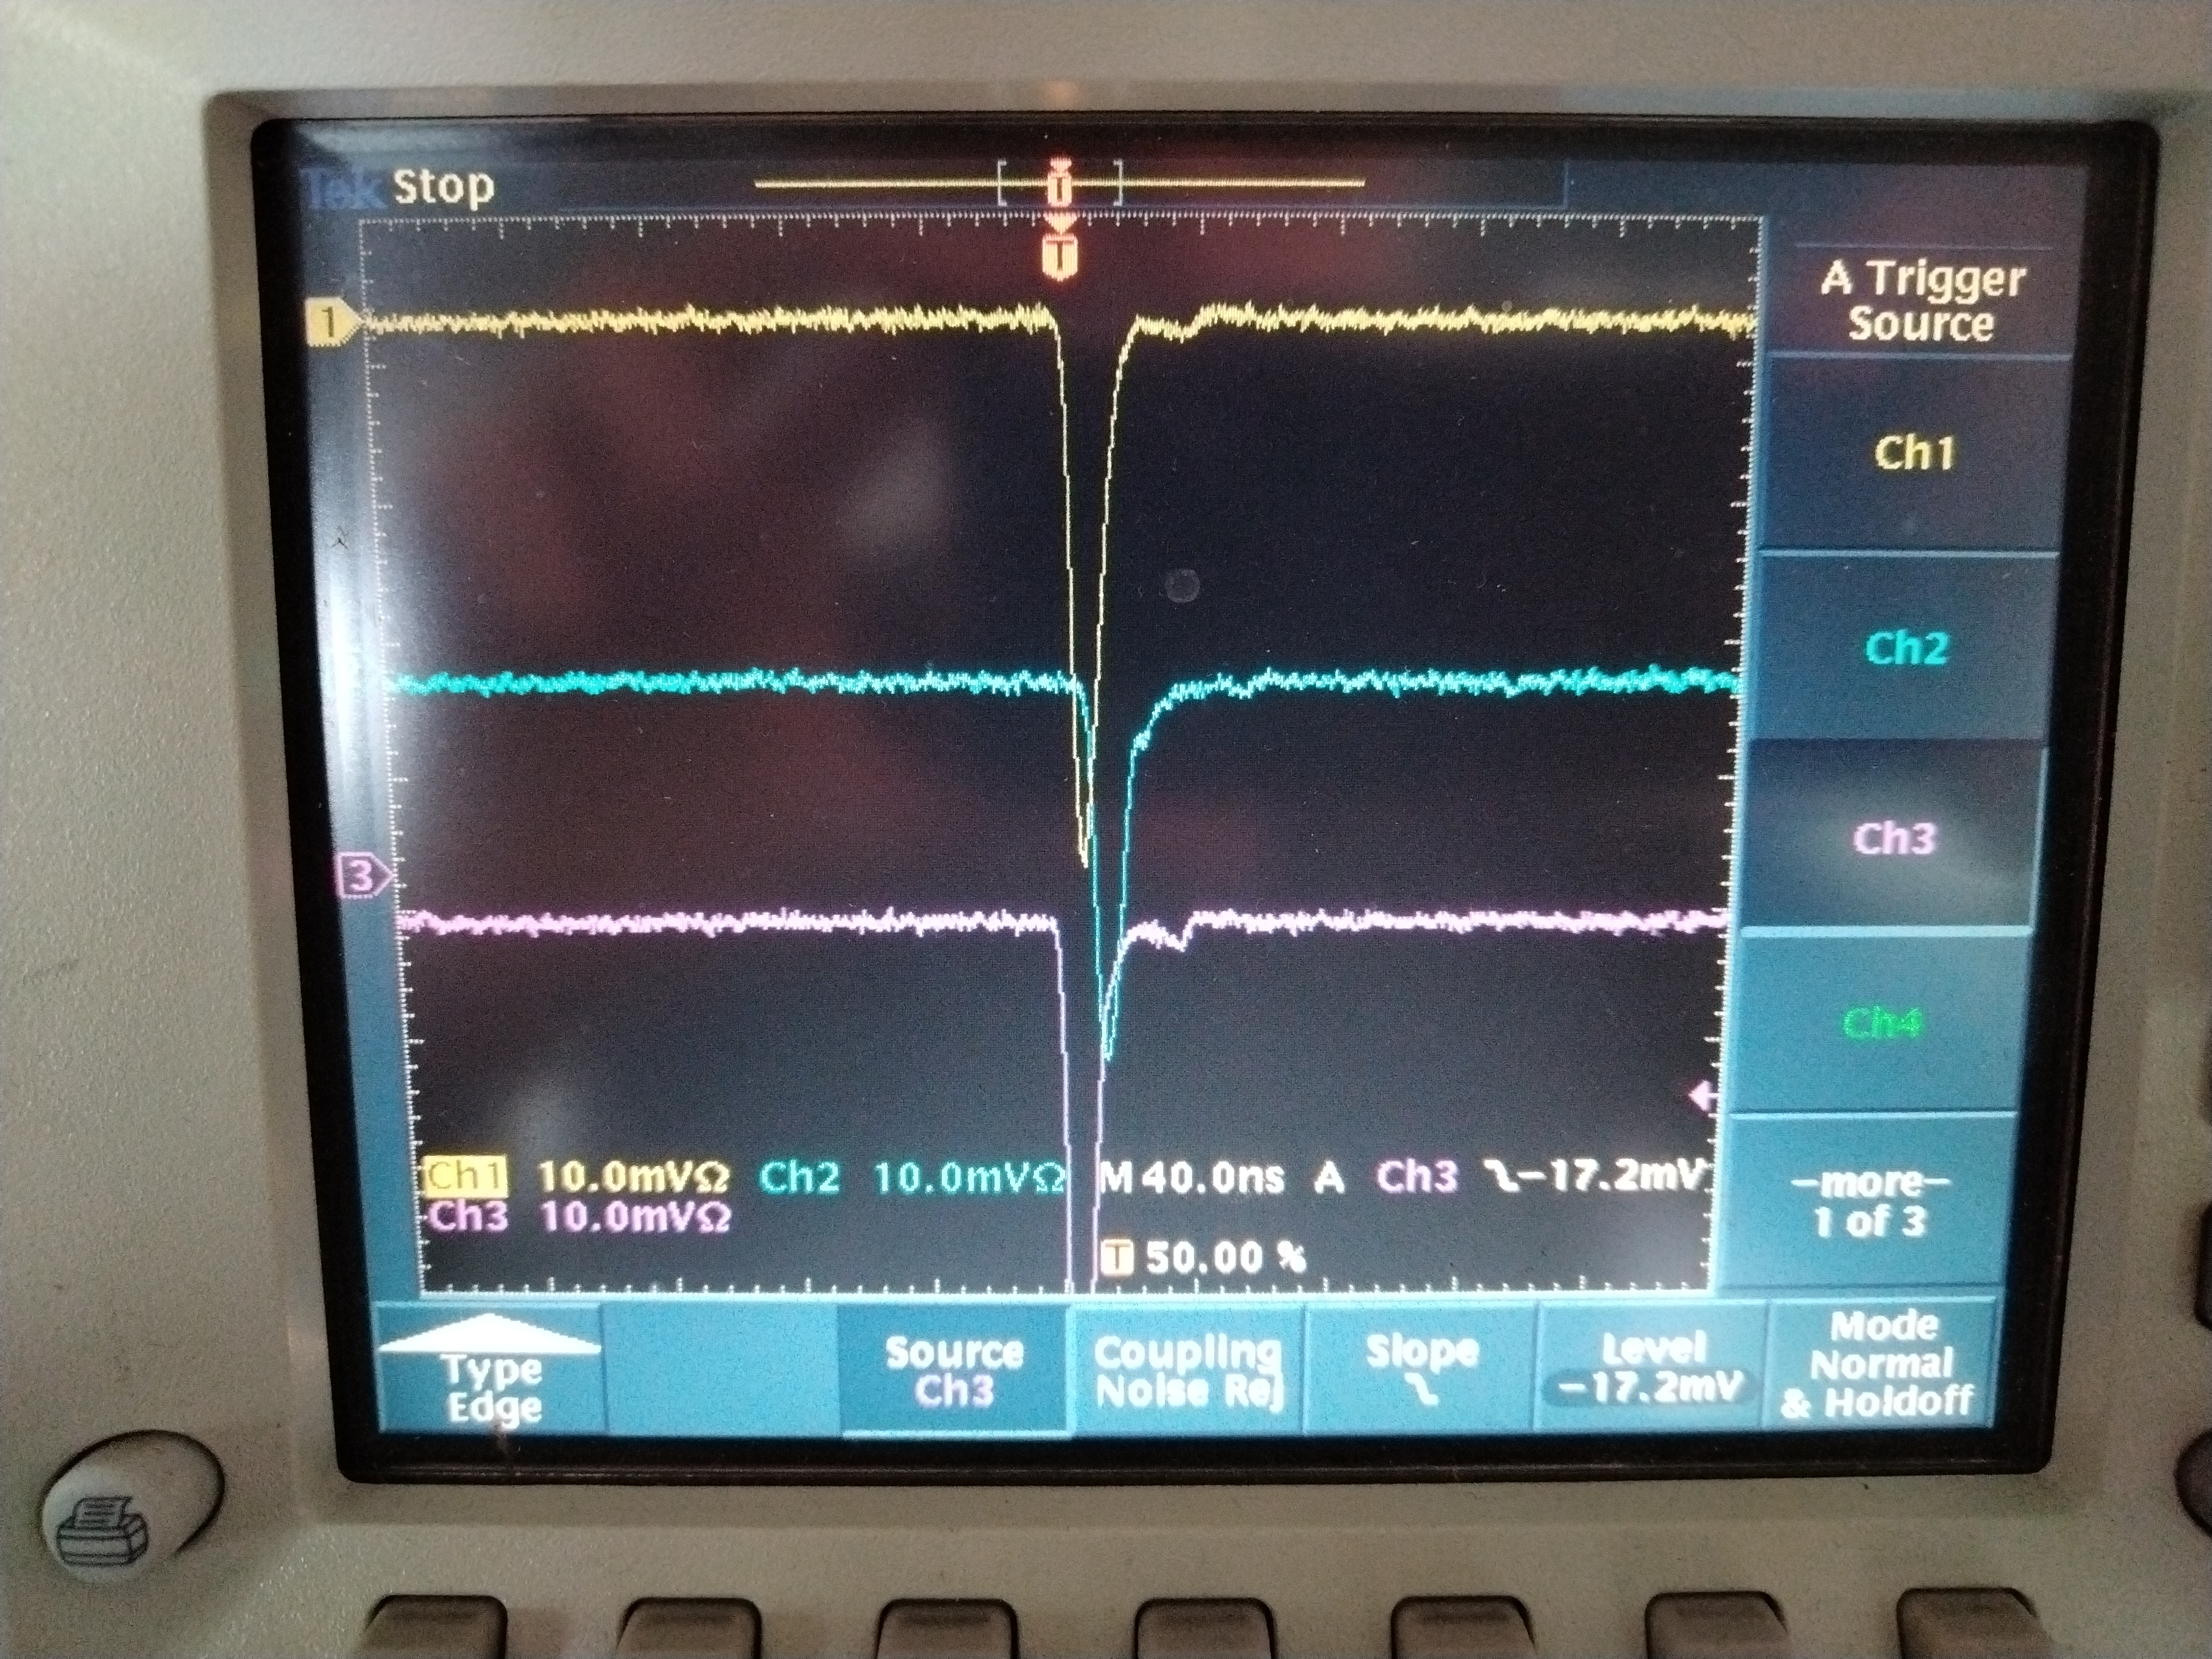
\includegraphics[width = 0.5\textwidth]{Analysis/IMG_20221027_170925.jpg} 
\end{figure}

The same procedure was followed also for detector A, made by 8 PMTs. We analyzed 4 pmt at a time, having the NINO board available with only 4 channels. The same attenuation scan performed for detector B was done:

\newpage
\begin{figure}[hbtp]
\centering
\includegraphics[width = 0.5\textwidth]{Analysis/AttenuationA(4-7).pdf}
\caption{Attenuation scan for Detector A}
\end{figure}

For these 4 pmt we are able to observe 


We took as above 10 acquisitions 1 minute long:

\begin{center}
\begin{tabular}{|c|c|c|c|c|}
\hline 
pmt & 2 & 1 & 0 & 4 (in coincidence) \\ 
\hline 
1 & 91 & 51 & 50 & 27 \\ 
\hline 
2 & 86 & 61 & 50 & 7 \\ 
\hline 
3 & 58 & 48 & 45 & 18 \\ 
\hline 
4 & 95 & 62 & 41 & 29 \\ 
\hline 
5 & 69 & 60 & 50 & 21 \\ 
\hline 
6 & 85 & 57 & 45 & 19 \\ 
\hline 
7 & 66 & 51 & 46 & 28 \\ 
\hline 
8 & 74 & 51 & 48 & 22 \\ 
\hline 
9 & 77 & 43 & 45 & 17 \\ 
\hline 
10 & 62 & 44 & 50 & 29 \\ 
\hline 
\end{tabular} 
\end{center}

\begin{equation*}
\begin{split}
\mu_{2} = 76.3 \qquad \sigma^{2} = 160  \\
\mu_{1} = 52.8 \qquad \sigma^{2} = 47.5 \\
\mu_{0} = 47.0 \qquad \sigma^{2} = 9.6  \\
\mu_{4} = 21.7 \qquad \sigma^{2} = 48.2 \\
\end{split}
\end{equation*}

For these 4 pmts , the variance of the sample changes significantly from what was observed earlier. We repot in this table the correlation matrix:

\begin{center}
\begin{tabular}{|c|c|c|c|c|}
\hline 
pmt: & 4 & 0 & 1 & 2 \\ 
\hline 
4 	 & 1 & -0.18  & -0.21  & -0.06  \\ 
\hline 
0 	 & -0.18  & 1 & -0.10  & -0.22  \\ 
\hline 
1    & -0.21  & -0.10  & 1 & 0.56  \\ 
\hline 
2    & -0.06 & -0.22  & 0.56  & 1 \\ 
\hline 
\end{tabular} 
\end{center}

Here we observe correlation that with negative sign, which are not expected. Also the correlatio between the pmt in coincidence are negative.
If we try to perform a gosset test, we obtain:

\begingroup
\setlength{\tabcolsep}{8pt} % Default value: 6pt
\renewcommand{\arraystretch}{1.2} % Default value: 1
\begin{center}
\begin{tabular}{|c|c|c|c|c|}
\hline 
Pmt: & 2 & 1 & 0 & pmt in coincidence \\ 
\hline
$\chi^{2}_{9}$ & 19.6 & 8.30 & 1.90 & 39.5\\ 
\hline
\end{tabular} 
\end{center}
\endgroup
\smallskip

The expected error for the result of this test is $\sigma = \sqrt{2*(n-1)} \simeq 4$. In this case we are observing 3 values that are $2\cdot \sigma $ far from the expected value. All this consideration indicate that the attenuation, or something in the DAQ program is not correctly set. 

\section{Analysis}

One of the main goal for this experiment was to measure the well know trasverse asymmetry of $^{12}C$, already measured before, as a test for the new electronic system. Previous measurements of the Transverse asymmetry have been performed for a carbon target. For this beam-time, the two spektrometers were placed at an angle such that the $Q^{2}$ values of the scattered electron is:

\begin{flushleft}
\begin{align*}
& Spektrometer A : \qquad Q^{2} = \SI{0.041337}{\giga \electronvolt} \qquad \textnormal{without Cut} \\
& Spektrometer A : \qquad Q^{2} = \SI{0.0394513}{\giga \electronvolt} \qquad \textnormal{with Cut} \\
& Spektrometer B : \qquad Q^{2} = \SI{0.0404771}{\giga \electronvolt} \qquad \textnormal{without Cut} \\
& Spektrometer B : \qquad Q^{2} = \SI{0.0405843}{\giga \electronvolt} \qquad \textnormal{with Cut} 
\end{align*} 
\end{flushleft}

The $Q^{2}$ values is the same of the last measurement performed at MAMI, and is measured with and without rejecting the inelastic electrons. 



\subsection{Alignment of the scattering plane}

\subsection{Calibration of the VFCs monitors}
Maybe it's important to divide this sections in two different part: the first part where I explain the Vfc convert the input voltage signal to a digital signal. In the second part just mention how we tuned the resistences (for X,Y monitors directly at the output signal with the oscilloscope, while for I21 and I13 monitors we used the data, so I'm able to produce plots only for the second ones).

\subsection{Calibration of the PIMO monitors}

For the calibration of the X Y monitors, we used two target made by three carbon wires at a certain distance from each other, aligned horizontaly and vertically. The distance between the two center of the external wires is $ d_{horizontal} = \SI{2.38}{\milli \meter}$ for the target alligned horizontally and $d_{vertical} = \SI{2.33}{\milli \meter}$ for the other one.
When the horizontal wires target is cetered, we turn on the beam, and we take some data slowly changing the horizontal beam direction. The beam direction is changed by MAMI operators, varying the Magnetic field of the \textit{Wobbler 16} magnets (\ref{fig:BeamLine}):

\begin{figure}[hbtp]
\centering
\includegraphics[scale=0.4]{figures/XYMOCalibBeamLine.svg.pdf}
\caption{Beam line scheme.}
\label{fig:BeamLine}
\end{figure}


 Then we repeat the same procedure with the other target, for the vertical direction. We observe that the pmts counts increase to a maximum, that is reached when the beam spot is centered on the carbon wire, and then decrease until the next carbon wire is hit by the beam.\\
We plot the pmt data \textit{versus} the $X25,X21,Y25,Y21$, given in $\SI{}{\volt}$. 
Given that we know the real distance between the two external wires, we can obtain the correct scaling factors to calculate the X and Y position values ​​of the beam. To identify the three peaks in of the carbon target, we fit the data using a gaussian model (see \ref{fig:HorizontalCalibration}). The mean $\mu$ represents the center of the wire, given in $\SI{}{\volt}$.
Looking at the Beam line, we assume that the beam travels in a straight line. Let's consider the \textit{Wobbler 16} magnet the "$0$" of a coordinate system, with the $z$ axis pointing to the target (left direction in the beam scheme). The Beam parameters are measured by the Monitors $X/Y_{21}, X/Y_{25}$, which are located at some distance respect to the target. Suppose we are working only with the $Y_{25}$ monitor (the procedure is the same for the others). The Beam $y$ position is described by:

\begin{align*}
y_{beam} = m \cdot (z - z_{wobbler 16})
\end{align*}

In the scheme \ref{fig:BeamLine} we easily compute the distance between the $Y_{25}$ monitor and the \textit{wobbler 16} magnet, so we have the slope $m$. The Position on the target is given by $Y_{target} = m \cdot Z_{target}$. With these simple equations then:

\begin{equation}
c_{Y25} = \dfrac{d_{vertical} [\SI{}{\milli \meter}]}{ Y_{target}} 
\end{equation}

$c_{Y25}$ indicates the scaling factor of the monitor. With these values the Analysis program compute the correct beam position, and from that the incident angles in the $x,y$ directions, which are needed later for the analysis.

\begin{figure}[hbtp]
\centering
\includegraphics[width=0.4\textwidth]{Analysis/HorizontalCalibration.png}
\caption{•}
\label{fig:HorizontalCalibration}
\end{figure}

All this procedure can be easely checked if we plot now the $X$ and $Y$ position for the same two runs of data acquired with the wires. After placing the scaling factors obtained in the standard configuration file, we run the analysis another time and the physical values were computed \ref{fig:CheckHori}

\begin{figure}[hbtp]
\centering
\includegraphics[width=0.45\textwidth]{Analysis/XcheckB.png} 
\includegraphics[width=0.45\textwidth]{Analysis/XcheckA.png}
\caption{plot of the pmt Count against the physical values computed by the analysis program. Now the position of the three peaks correspond to the expected values measured for the target.}
\label{fig:CheckHori}
\end{figure}


\subsection{Current and ENMO monitors}

For the current monitors I13 and I21, we perform the calibration changing the current of the beam and observing the output values of the monitors (Voltage values). The we perform a fit (for the beam current, we used the nominal values that we communicate to MAMI, has the values for the x-axis).

\begin{figure}[hbtp]
\centering
\includegraphics[width = 0.45\textwidth]{Analysis/I13_Calibration.png}
\includegraphics[width = 0.45\textwidth]{Analysis/I21_Calibration.png} 
\caption{•}
\end{figure}

For the two monitors we are able to compute the offset and scale factor:

\begin{equation}
\begin{split}
I^{volt}_{13} = m_{13} \cdot I^{Nom}_{13} + q_{13}\\
c_{13} = \frac{1}{m} \qquad offset = -\frac{q_{13}}{m}
\end{split}
\end{equation}

The same formula for current monitor I21.

The Enmo calibration is performed in a different way from the other monitors. The polarity signal is sent to MAMI, and they produce a signal for the ENMO that somehow (need to investigate exactly how they do that) shows a difference between the first two subevents and the last two. This difference is equal (nominal) to $\SI{22.6}{\kilo \electronvolt}$. The idea now is to produce an histogram for the quantity $\delta E$ (with $E_{18}$ being the energy monitor):

\begin{equation*}
\delta E = \frac{E_{18}[2] + E_{18}[3]}{2} - \frac{E_{18}[0] + E_{18}[1]}{2} 
\end{equation*}

The data should be distributed with a peak around $\SI{22.6}{\kilo \electronvolt}$. To obtain the correct scaling factor for the values stored in the data tree we plot the voltage values mesured by the ENMO monitor.
3 runs of data where taken with different Beam current, to study the dependence of the measured quantity from the beam current. From the mean of the distribution it is possible to exstimate the scaling factor for the ENMO monitors, obtaining the physical quantity in the following way:

\begin{equation*}
C_{E18} = \frac{\SI{22.6}{\kilo \electronvolt}}{\overline{\delta E}}
\end{equation*}

\begin{figure}[hbtp]
\centering
\includegraphics[width = 0.45\textwidth]{Analysis/ENMOvoltage20.pdf}
\includegraphics[width = 0.45\textwidth]{Analysis/ENMOvoltage15.pdf} 
\caption{$\delta E$ for 20 $\SI{20}{\micro \ampere}$}
\end{figure}

Taking the average over $E_{18}$ voltage values, and using the formula above, we obtain the coefficient $C_{E18}$. To take care of the current depencende of the monitors, the scaling factor to be placed in the standard.config file is: $C_{E18} \overline{I}_{\mu A}$.
The calibration was performed taking three short acquisitions with different beam current : $\SI{20}{\micro \ampere}$, $\SI{15}{\micro \ampere}$ and a run without beam. 

\begin{figure}[hbtp]
\centering
\includegraphics[width = 0.5\textwidth]{Analysis/E18_Calibration.png}
\caption{Calibration of ENMO monitor}
\end{figure}

From this we obtain the value $scaling_{E18} = -1595.2$, to obtain the physical quantity from the analysis. As a final check the final histogram for the physical quantity is shown:

\begin{figure}[hbtp]
\centering
\includegraphics[width = 0.45\textwidth]{Analysis/ENMOCheck20.pdf}
\includegraphics[width = 0.45\textwidth]{Analysis/ENMOCheck15.pdf} 
\caption{Plot for the physical quantities computed in the data tree, for two different current of the beam (on the left $\SI{20}{\micro \ampere}$, $\SI{15}{\micro \ampere}$ on the right)}
\end{figure}



\subsection{Calibration of the pmts}

{\bfseries Here it's important to show the plots I made during the beam time. I have to mention the Leo tecniques for the correct interpretation of counts vs attenuation.}

During the beam time, several scans in attenuation were performed, before switching MAMI to produce the polarized beam, to choose the best working point for the PMTS of the detectors. The same procedure used in the laboratory was followed, starting from low attenuation and raising up the values. It's possible to get a simple model to describe the particular shape of the following plot taking into account simple assumptions about the type of electrical noise that affect the Nino board, and the \textit{pdf} of the signal produced by the PMTS.
The main assumption ("this is not a true assumption, Anselm has a plot of the digitalize charge that proves that") is that the signal amplitude, in $\SI{}{\milli \volt}$ collected by the Nino board is well described by a gaussian distribution, and for signal with low amplitude, we expect to be well described by an uniform distribution. Just to visualize, let's suppose that the distribution of the signal amplitude collected is of this type (\ref{fig:PDF}) (the following figure is just an example, the values ​​do not describe the data collected):

\begin{figure}[hbtp]
\centering
\includegraphics[width = 0.40\textwidth]{Analysis/distribution.pdf}
\caption{Example of the expected distribution of the PMTs output signal}
\label{fig:PDF}
\end{figure}

The probability for a signal to pass the selection is equal to the probability of being in above the threshold, that is the complementary cumulative of the gaussian distribution (probability of being in the right tail):

\begin{align*}
P(signal > thr) = 1 - \Phi(x) = \dfrac{1 - Erf(\dfrac{x_{thr} - x_{0}}{\sqrt{2} \sigma })}{2}
\end{align*}

Once we reach the uniform zone, the probability of an even being selected is proportional to the area of the rectangle, which increases linearly decreasing the threshold. Considering the normalization factor, it is straightfoward to fit the data with a model of this type:

\begin{equation}
\begin{split}
N(att) = N_{0} \cdot \dfrac{1 + Erf(\dfrac{x_{thr} - x_{0}}{\sqrt{2} \sigma })}{2} \qquad \text{if} \quad att < C  \\
N(att) = N(C) + m \cdot (att - C) \qquad \text{if} \quad att > C
\end{split}
\end{equation}

For the detector B we show the result assuming our model: 

\begin{figure}[hbtp]
\centering
\subfloat[][\emph{Attenuation scan for the pmts of detector B} \label{fig:FitAtt}]
{\includegraphics[width = 0.5\textwidth]{Analysis/Fit_attenuation.pdf}}
\subfloat[][\emph{Recostructed spectra for Detector B, notice that we have \textit{Attenuation} values in the x axis, therefore right and left are swapped with respect to the graph \ref{fig:PDF}.} \label{fig:Spectra}]
{\includegraphics[scale = 0.5]{Analysis/Bspectra.pdf}}
\end{figure}

From the fit we obtain three valus for the signal Peak, given in attenuaton units.
We can check the idea behind this, visualizing the pmt count in a different way. In this plot (\ref{fig:FitAtt}) there is a discrete differentiation of the data showed in (\ref{fig:Spectra}). This plot represents roughly the signal spectra of the signal (we report for brevity only the plot for detector B, for Detector A the same procedure was followed). 
We can see that our assumption is not far from what we see, except for the fact that we are not able to identify the linear area. This is not very importat, sice we have to indenty properly a good point to select all the real signals from the scattered electrons, rejecting the noise. Furthermore, if we look at the plot (), we can understand this behaviour looking that the threshold does not scale linearly with changing the attenuation value, for high values of attenuation, the threshold falls quickly at zero.

 
From the NINO documentation, it's possible to confront these values with 

\newpage
\subsection{Autocalibration procedure}

\begin{figure}[!h]
\centering
\includegraphics[width = 0.75\textwidth]{Analysis/Autocalib/Current.pdf} 
\end{figure}

\newpage
\subsection{Rates on lead}

{\bfseries This section is straightforward. Basically I have to show the single plot of the pmts counts vs. beam current for lead target. However it's possible to do some preliminary studies, for example to calculate the time needed for measuring the asymmetry on lead with a certain error and maybe check from Mott cross section that the observed rate are fine.}

\begin{figure}[hbtp]
\centering
\includegraphics[width = 0.45\textwidth]{Analysis/Rates_on_lead.png}
\includegraphics[width = 0.45\textwidth]{Analysis/Rates_on_leadB.png}
\caption{Rates on lead Target, for Detector A (left)}
\end{figure}

\newpage

\section{Asymmetry on Carbon}

\section{Model for fitting the data}
Here I have to explain the model used for describing the data, so the problem of the false asymmetry induced by variations in beam position, angle, current and energy.\bigskip

One of the problems of the measurement is to take into consideration the various contributions that can change the value of the asymmetry measured by the experimental apparatus. The raw values of the asymmetry can be affected by the variation of the beam parameters during the time. Let's summarize quickly all these effects:
\begin{itemize}
\item the pmts counts  can depend on the $(x,y)$ impact position of the beam on the target
\item the variations of the incident angles $\theta_{x}$and $\theta_{y}$ on the target.
\item the uncertain associated with the energy of the Beam, a change in the energy associated with the polarization of the beam leads to different rates for the cross section
\item the uncertain associated with the current of the Beam, in particular a change due to the 
efficiency of the source in producing electrons polarized in the two opposite directions
\end{itemize}

All this quantity can influence the asymmetry measured by the pmts, considering also that the expected asymmetry is in the order of ten part per million, and small asymmetry introduced by fluctuations on the beam parameters are not negligible. Correcting directly the false asymmetries that rise from those uncertainties is a tough task, and it's more easy to adopt a different strategy respect to proceed to the analytical/numerical calculation of each of them . Knowing that the beam parameters produced by Mami are quite stable over the time, we can assume that the measured asymmetry are well described by a linear model as the following:

\begin{equation}
Asym = A_{physical} \cdot P + \delta_{I} + A_{x} \delta x + A_{y} \delta y + A_{\theta_{x}} \delta \theta_{x} + A_{\theta_{y}} \delta \theta_{y}+ A_{E} \delta E 
\end{equation}

$A_{physical}$ is the aim of the experiment, $A_{x}$ and $A_{y}$ are the asymmetries induced by the variation of the posizion of the beam, $A_{\theta_{x}}$ and $A_{\theta_{y}}$ are the asymmetry associated to angles, $A_{E}$ is the asymmetry associated to the beam energy. 
The relevant assumption is that, for small variation of the beam, the false asymmetry are linearly dependent on the Beam uncertainties (that are $\delta x, \delta y, \delta \theta_{x}, \delta \theta_{y}, delta_{E}$), so a first order approximation seems valid.\\
We must clarify now what we mean with $\delta x, \delta y, \delta \theta_{x}, \delta \theta_{y}, delta_{E}$. Resuming the event structure, that we discussed in \ref{FirstDescription}, we have a sequence of 4 different sub-events, with a polarization pattern that is randomly selected between $\uparrow,\downarrow,\downarrow, \uparrow$ and $\downarrow,\uparrow,\uparrow,\downarrow$. During the $\SI{20}{\milli \second}$ ot time lenght of each sub-event, the vfcs make a single measurement of the beam, and the data are saved in the data tree. The task of the analysis program is to use this raw data to calculate the relevant parameters for the analysis. Because we are working with asymmetries, the absolute values of the parameters listed above is not relevant, instead what is relevant are the differencies correlated with polarization state of the beam. Assuming this, $\delta x, \delta y, \delta \theta_{x}, \delta \theta_{y}, delta_{E}$ are replaced with :

\begin{equation}
\begin{split}
\delta {x} & = \Bigl(\dfrac{X_{\uparrow}(1) + X_{\uparrow}(2)}{2}\Bigl)  - \Bigl(\dfrac{X_{\downarrow}(1) + X_{\downarrow}(2)}{2}\Bigl)\\
\delta {y} & = \Bigl(\dfrac{Y_{\uparrow}(1) + Y_{\uparrow}(2)}{2}\Bigl)  - \Bigl(\dfrac{Y_{\downarrow}(1) + Y_{\downarrow}(2)}{2}\Bigl)\\
\delta {E} & = \Bigl(\dfrac{E_{\uparrow}(1) + E_{\uparrow}(2)}{2}\Bigl)  - \Bigl(\dfrac{E_{\downarrow}(1) + E_{\downarrow}(2)}{2}\Bigl)\\
\delta {\theta_{x}} & = \Bigl( \dfrac{\theta_{x,\uparrow}(1) + \theta_{x,\uparrow}(2)}{2} \Bigl) - \Bigl(\dfrac{\theta_{x,\downarrow}(1) + \theta_{x,\downarrow}(2)}{2} \Bigl)\\
\delta {\theta_{y}} & = \Bigl( \dfrac{\theta_{y,\uparrow}(1) + \theta_{y,\uparrow}(2)}{2} \Bigl) - \Bigl(\dfrac{\theta_{y,\downarrow}(1) + \theta_{y,\downarrow}(2)}{2} \Bigl)\\ 
\end{split}
\end{equation}

Each value represent the difference between the mean values over the two different polarization state.

\subsection{Data selection and Fit}

After all the calibration are performed, the analysis program is ready to produce the datafiles suitable to analyze the asymmetry data for Carbon. \\
The Data file that are produced from the binary files are simply files in txt format, where the data are stored in columns. Before proceeding with the linear fit, however, it is necessary to visualize the data to check that there are no anomalous behaviors. In fact the data can contain moments of loss of the beam burrent and sudden interruptions, loss of polarization of the beam and even setting errors by MAMI operators can affect the experiment. Carbon data were taken from November 2nd to 4th, and consist of $28$ runs, each $1$ hour long.
The first step is to observe the pmt counts and the current trend, in order to be able to identify sudden interruptions of the beam. Here we show the trend over time for the series runs: 

\begin{figure}[hbtp]
\centering
\subfloat[][\emph{Pmt count trend versus time.In black A0, in green B0} \label{fig::CountTrend}]{
\includegraphics[width = 0.45\textwidth]{Analysis/Dataselection/BeamExample.pdf}}
\subfloat[][\emph{Asymmetry trend for pmt A0} \label{fig::AsymTrend}]{
\includegraphics[width = 0.45\textwidth]{Analysis/Dataselection/AsymmetryTrend.pdf}}
\end{figure}

This plot show that after 10 h of data acquisition the Pmt counts (\ref{fig::CountTrend}) dropped rapidly. If we show the current trend over the time (\ref{fig::CurrentTrend}) we do not see a corresponding decrease in beam intensity. Also the $x,y$ position (\ref{fig::PositionTrend}) and the energy monitor of the beam do not show a strange behavior. So we reject the possibility that at some point one of the stabilization device of the beam stop working. One of the possibilities is that something happen inside the two spectrometers. From the pmt counts we can suggest that the scattered electrons were not hitting our fused-silica detector,
in fact for pmt B0 we observe roughly 0 counts, and for pmt A0 $20000$ counts, which is compatible with the noisy offset of that pmt. This consideration strongly suggest as to reject those data from the analysis.\\
Apart from this, we observe in (\ref{analysis}) two steepy variations of the asymmetry around $13.5 h$ and $19 h$. For these data is quite simple to explain why should be rejected: we observe the same steepy variations also for the positions, so in this case the beam was not correctly aligned to the target.

\begin{figure}[hbtp]
\centering
\subfloat[][\emph{Current trend over time.} \label{fig::CurrentTrend}]{
\includegraphics[width = 0.45 \textwidth]{Analysis/Dataselection/CurrentTrend.pdf}}
\subfloat[][\emph{$X,Y$ beam position over time} \label{fig::PositionTrend}]{
\includegraphics[width = 0.45\textwidth]{Analysis/Dataselection/XYtrend.pdf} }
\end{figure}

After this first data selection, we check the correlated-difference data, which will be later used as variables for the fit. We produced histograms for all this quantites, that we remember are computed by the analysis program with the formula:

\begin{align*}
\delta x =  \frac{(x_{up,1} + x_{up,2})}{2} - \frac{(x_{down,1} + x_{down,2})}{2}
\end{align*}

We expect, if the stabilization of the beam is correctly set, that those quantities are gaussian distributed. A maximum likelihood fit with a Gaussian model is performed for each beam parameter, with Likelihood Ratio for the goodness of fit (gof). The statistic for the gof is:

\begin{align*}
\lambda(x) = 2 \sum_{i}^{n} (f_{i}(\mu) - k_{i}(1 + log(\frac{f_{i}(\mu)}{k_{i}})))
\end{align*}  

$\mu$ are the parameters of the \textit{pdf}, that are mean and variance of the gaussian, and $f_{i}(\mu)$ and $k_{i}$ are respectively the expected value for the i-nth bin and the observed value for the i-nth bin.

\newpage

\begin{figure}
\centering 
\subfloat[][\emph{$X$ position correlated difference}]{
\includegraphics[width = 0.3\textwidth]{Analysis/Dataselection/X.pdf}} 
\subfloat[][\emph{$Y$ position correlated difference}]{
\includegraphics[width = 0.3\textwidth]{Analysis/Dataselection/Y.pdf}}
\subfloat[][\emph{$\theta_{x}$ correlated difference}]{
\includegraphics[width = 0.3\textwidth]{Analysis/Dataselection/Xp.pdf}} \\
\subfloat[][\emph{$\theta_{y}$ correlated difference}]{
\includegraphics[width = 0.3\textwidth]{Analysis/Dataselection/Yp.pdf}}
\subfloat[][\emph{Energy correlated difference}]{
\includegraphics[width = 0.3\textwidth]{Analysis/Dataselection/ENMO.pdf}}
\end{figure}

Looking at the histograms, we see that the beam correlated-difference values are centered around zero, the result are reported below:

\begin{center}
\begin{tabular}{|c|c|c|c|c|c|}
\hline 
\rule[-1ex]{0pt}{2.5ex} & $X [\mu m]$ & $Y[\mu m]$ & $Xp [\mu rad]$ & $Yp [\mu rad]$ & $E [eV]$ \\ 
\hline 
\rule[-1ex]{0pt}{2.5ex} $\mu$ & $1.31 \cdot 10^{-3}$ & $2.4 \cdot 10^{-4}$ & $3.2 \cdot 10^{-8} $ & $3.6 \cdot 10^{-9}$ & $0.0013$ \\ 
\hline 
\rule[-1ex]{0pt}{2.5ex} $sigma$ & $3.7 \cdot 10^{-1}$ & $2.9 \cdot 10^{-2}$ & $ 1.9 \cdot 10^{-5} $ & $6.5 \cdot 10^{-6}$ & $0.38$ \\ 
\hline 
\end{tabular} 
\end{center}

these results are encouraging, the stabilization of the beam has meant that only small differences are observed within an event for each monitor. This means that, unless the values for the false asymmetries are not very large, the effect of the beam variation are small.
Before proceeding with the fit, we observe how the asymmetry evolves as a function of time.

\begin{figure}[hbtp]
\centering
\includegraphics[width = 0.8 \textwidth]{Analysis/Dataselection/AveragedAsymmetry.pdf}
\caption{Plot of the Asymmetry versus time. For a point time $t_{1}$, we plot the mean over all the asymmetries collected from $t = 0$ to $t = t_{1}$. Each line represents the asymmetries measured for a specific pmt (in \textcolor{blue}{blue} detector B and in \textcolor{red}{red} detector A). The values are corrected for the beam polarization, multiplying by $\frac{1}{p}$. We plot also the error, which is one standard deviation $\sigma$ from the mean.}
\end{figure}

In this figure we plot the average of the asymmetries for each pmt, carried out from the beginning up to the instant $t$. The data shown are corrected with the percentage of polarization of the beam ($p \simeq = 0.79$). From this it can be seen how the asymmetry evolves as time increases. If there are still outliers data, we can directly check from this plot there a steepy variation in the data. 


When all the calibrations are performed, it is possible to proceed to generate the datafiles fot the fit program.

For a better visualization of the data, especially to observe the dependence of the asymmetry on the Beam parameters measured, it is useful to take the average asymmetry at regular intervals. From the raw plots of the asymmetries (see below \ref{fig:asyvsparam}), it is clear that the statistical error associated to the asymmetry is the main one, and it's not possible to identify a linear dependence. In the meantime, this plot shows that there is a difference in sign between the values ​​measured by the two detectors, and that at the end the averaged result are on the same order of magnitude of what we expect $\pm 20 \quad ppm$ at our scattering angle $\theta$. These results, coupled with the fact that the correlated differences in beam values ​​are small, suggest that the contribution of false asymmetries is limited.

\begin{figure}[hbtp]
\centering
\includegraphics[width = 0.5\textwidth]{Analysis/Asym_vs_monitor.png}
\caption{Asymmetries vs. Beam parameters}
\label{fig:asyvsparam}
\end{figure}

In some plots (X,Y and I) we can identify equally spaced cluster of data. So we decide to compute the averaged asymmetry for each cluster we were able to identify. 
In the following plots we decided to apply some cuts to the data, selecting only the events where the values of all the monitor are less then 3 standard deviation far from the mean. In all the figures the asymmetries are multiplied by a factor of $1e6$ to have the result in ppm (so each y-axis is in ppm). 

\begin{align*}
(x_{monitor} - \overline{x}_{monitor}) \leq 3 \cdot \sigma_{X}
\end{align*}

For each monitor we use the \textit{curve fit} function of the python library \text{scipy} to fit the data. Each Beam parameter is treated separately now, so in principle we are ignoring possible effect of correlation between the X-values (however, from the correlation matrix    \textit{write that somewhere} the effects are negligible)  

\newpage
\begin{figure}[hbtp]
\centering
\subfloat[][\emph{Asymmetries [ppm] vs X position [$mm$]}]
	{\includegraphics[width = 0.45\textwidth]{Analysis/clustering_XB.pdf}} \quad
\subfloat[][\emph{Asymmetries [ppm] vs Y position[$mm$]}]
	{\includegraphics[width = 0.45\textwidth]{Analysis/clustering_YB.pdf}} \\
\subfloat[][\emph{Asymmetries [ppm] vs $\theta_{x}$ angle [$rad$]}]
	{\includegraphics[width = 0.45\textwidth]{Analysis/clustering_XpB.pdf}} \quad
\subfloat[][\emph{Asymmetries [ppm] vs $\theta_{y}$ angle [$rad$]}]
	{\includegraphics[width = 0.45\textwidth]{Analysis/clustering_YpB.pdf}} \\
\subfloat[][\emph{Asymmetries [ppm] vs E [$keV$]}]
	{\includegraphics[width = 0.45\textwidth]{Analysis/clustering_EB.pdf}} \quad
\subfloat[][\emph{Asymmetries [ppm] vs I current [arb.unit]}]
	{\includegraphics[width = 0.45\textwidth]{Analysis/clustering_IB.pdf}} \quad
\label{fig:averageAsym}
\end{figure}

\begin{figure}[hbtp]
\centering
\subfloat[][\emph{Asymmetries [ppm] vs X position [$mm$]}]
	{\includegraphics[width = 0.45\textwidth]{Analysis/clustering_XA.pdf}} \quad
\subfloat[][\emph{Asymmetries [ppm] vs Y position[$mm$]}]
	{\includegraphics[width = 0.45\textwidth]{Analysis/clustering_YA.pdf}} \\
\subfloat[][\emph{Asymmetries [ppm] vs $\theta_{x}$ angle [$rad$]}]
	{\includegraphics[width = 0.45\textwidth]{Analysis/clustering_XpA.pdf}} \quad
%\subfloat[][\emph{Asymmetries [ppm] vs $\theta_{y}$ angle [$rad$]}]
%	{\includegraphics[width = 0.45\textwidth]{Analysis/clustering_YpB.pdf}} \\
%\subfloat[][\emph{Asymmetries [ppm] vs E [$keV$]}]
%	{\includegraphics[width = 0.45\textwidth]{Analysis/clustering_EB.pdf}} \quad
%\subfloat[][\emph{Asymmetries [ppm] vs I current [arb.unit]}]
%	{\includegraphics[width = 0.45\textwidth]{Analysis/clustering_IB.pdf}} \quad
\label{fig:averageAsym2}
\end{figure}


The error of each point is computed exploiting the same formula defined above (theory section; $N_{A/B}$ averaged pmt counts for each subevents and $n$ number of event in each interval):

\begin{align*}
\sigma_{Asym} = \dfrac{1}{\sqrt{2N_{A/B} \cdot n}}
\end{align*}

From this plots we can check if the linear model is good enough to descrive the depencence of out data and decide if the it should be useful to apply different cuts for certain beam parameters. We report now a first exstimation of the false asimmetries, later the data will be fitted without treat separately the beam parameters. From that we can learn the effects of the correlation between the data.

\begin{center}
\begin{tabular}{||c|c|c|c|c|}
\hline
pmt: & B0 & B1 & B2 & unit \\ 
\hline 
$\frac{dA}{dX} $  & $-66 \pm 37$ & $-65 \pm 37$ & $-80 \pm 47$ & $ \frac{ppm}{\SI{}{\micro \meter}}$\\ 
\hline 
$\frac{dA}{dY} $  & $34 \pm 219$  & $ 79 \pm 233$ & $ -213 \pm 219$ & $\frac{ppm}{\SI{}{\micro \meter} }$ \\ 
\hline 
$\frac{dA}{d\theta_{y}}$ & $-416 \pm 1181$  & $ -443 \pm 1227$ & $-1237 \pm 1130$ & $\frac{ppm}{\mu rad}$\\ 
\hline 
$\frac{dA}{d\theta_{x}}$ & $-672 \pm 297$ & $ -672 \pm 307 $ & $-845 \pm 380$ & $\frac{ppm}{\mu rad}$ \\ 
\hline 
$\frac{dA}{dE}$ & $ -0.004 \pm 0.016 $ & $-0.011 \pm 0.016 $ & $ - 0.044 \pm 0.018 $ & $\frac{ppm}{\SI{}{\kilo \electronvolt}}$\\ 
\hline
\end{tabular} 
\end{center}


\subsection{False asymmetries}
{\bfseries Seems that is possible to obtain rough estimates of the beam related asymmetries with the results from the fit. For Energy and position it's achievable, while for the angles it's quite hard (in principle sounds possible to perform an analytic calculation of the asymmetry related to the incident beam angle, however Anselm told me that quite often those results are in disagrement with the observed even in the sign!).}

Until now the values for the false asymmetries were threated as the parameters of the fit. In this section we will investigate how we can obtain another different exstimations, usefult to check the validity of all the process of analysis of the data.

For $\frac{dA}{dX}$ and $\frac{dA}{dY}$, we conceptually exploit the possibility of varying the position of the beam on the target, as we did during one of the calibration phases. Using the same \textit{wobbler 16} we asked MAMI to slowly change the beam position on the X and Y monitor. The change in position has the effect to modify the rates for the two detector, and from them it's possible to extract exstimate the two false asymmetries related to the beam position. Now we will see how the two quantities are related.
From the plot .. we see that the counts are scaling linearly with the beam position, so we assume that the $N$ are given by

\begin{align*}
N(x,...) = N_{0} + m \cdot (x - x_{0})
\end{align*}

it is clear that the linear model can't be alwaws good, at some point the electron will be deflected completely out of the detector, however for the small variation that the magnets are producing this can be assumed without risk. The we can try to compute the asymmetry for two different beam position $x_{1}$ and $x_{2}$:

\begin{equation}
\begin{split}
Asym = \dfrac{N(x_{1}) - N(x_{2})}{N(x_{1}) + N(x_{2})} = \dfrac{N_{0} + m \cdot (x_{1} - x_{0}) - N_{0} - m \cdot (x_{2} - x_{0})}{N(x_{1}) + N(x_{2})} =  \dfrac{m}{2 N_{0} + m \cdot (x_{1} +  x_{2}) - 2m x_{0}}(x_{1} -  x_{2})
\end{split}
\end{equation}

We can approximate the denominator deleting the term $ m \cdot (x_{1} +  x_{2})$ which should be small compared to $2N_{0}$. We end with:

\begin{equation}
Asym = \dfrac{m}{2N_{0} - 2mx_{0}}(x_{1} -  x_{2})
\end{equation}

The term in front of $(x_{1} - x_{2})$ can be compared to $\frac{dA}{dX}$. $x_{0}$ is arbitrary and can be set to 0. For $N_{0}$, the offset, we substitute the averaged value counts of each pmt for the polarized beam acquisitions ( we remind that the rate are collected during each $\SI{20}{\milli \second}$ time interval of each sub-event).\\
The data are reported in the table below:

\begin{center}
\begin{tabular}{|c|c|c|}
\hline 
Pmt & Detector A & Detector B \\ 
\hline 
pmt 0 & 84718 & 18925 \\ 
\hline 
pmt 1 & 96882 & 18815 \\ 
\hline 
pmt 2 & 80604 & 14807 \\ 
\hline 
pmt 3 & 65053 & \\ 
\hline 
pmt 4 & 45943 & \\ 
\hline 
pmt 5 & 46248 & \\ 
\hline 
pmt 6 & 37452 & \\ 
\hline 
pmt 7 & 25808 & \\ 
\hline 
\end{tabular} 
\end{center}
 
We report the values obtained with this new method ... 

\begin{figure}[hbtp]
\centering
\subfloat[][\emph{Plot for slow variation in $x$ direction for detector B.}]
{\includegraphics[scale=0.5]{Analysis/slowxVariation.pdf}}
\subfloat[][\emph{Plot for slow variation in $x$ direction for detector B.}]{\includegraphics[scale=0.5]{Analysis/slowyVariation.pdf} }
\end{figure}

We can investigate also the asymmetries related to the beam energy. For this one we can exploit the theoretical expression for the Mott cross-section, taking the derivative ...

We can investigate the Current asymmetries, because we have the autocalibration procedure, so from the scale factor we can check if the current asymmetri is compatible with $1$ as assumed or not.
\subsection{??Bootstrap??}

Although Anselm was against it, now seems possible to increase the precision of the mesurement with a procedure similar to a bootstrap. Instead of computing all the quantities inside a single event, it's possible to compute all the important quantities also between different events. In this scenario the statistics can be increased artificially as mutch as we want, with the same amount of data. Of course, it's also simple to abuse of this method, so we should restrict using only events next to each other. However seem reasonable and promising.





\chapter{Result} \label{result}

\commento{\begin{itemize}
\item asymemtries on carbon.
\item expected rates on lead.
\item false asymmetriies result.
\item average of the asymmetries for the pmts.
\item confront with the theory.
\end{itemize}}

In this chapter we report the result obtained for the data-analysis. First we report the averaged asymmetries with and without subtracting the pmt offset. From the asymmetry results, we can compute the factor $c$ as the ratio between the final asymmetries with and without subtracting the offset. The values can be directly confronted with the ones defined in \ref{Autocalib}. We see a good agreement. All the values are in reported in ppm (part-per-million).

\begin{table}[!ht]
\centering
\subfloat[][\emph{Asimmetries, with offset not subtracted.} \label{table:NotCorrected}]{ 
\begin{tabular}{c|c|c}
\hline
 PMT   &   Average &   $\sigma$ \\
\hline
 B0    &    -21.64 &      7.9 \\
 B1    &    -19.96 &      7.9 \\
 B2    &    -24.91 &      8.9 \\
 A0    &     18.83 &      3.7 \\
 A1    &     15.92 &      3.5 \\
 A2    &     18.8  &      3.8 \\
 A3    &     18.54 &      4.2 \\
 A4    &     20.47 &      5   \\
 A5    &     22.61 &      5   \\
 A6    &     18.45 &      5.6 \\
 A7    &     18.41 &      6.7 \\
\hline
\end{tabular}} \qquad
\subfloat[][\emph{Asymmetries with offsets subtracted}\label{table:OffsetCorrected}]{
\begin{tabular}{lrr} 
\hline
 PMT   &   Average &   \sigma \\
\hline
 B0    &    -22.46 &      7.9 \\
 B1    &    -20.73 &      7.9 \\
 B2    &    -25.33 &      8.9 \\
 A0    &     24.25 &      3.7 \\
 A1    &     21.6  &      3.5 \\
 A2    &     24.25 &      3.8 \\
 A3    &     22.58 &      4.2 \\
 A4    &     23.53 &      5   \\
 A5    &     25.88 &      5   \\
 A6    &     20.86 &      5.6 \\
 A7    &     19.89 &      6.7 \\
\hline
\end{tabular}}
\qquad
\subfloat[][\emph{$c$ factor, as defined in \ref{eq:Systematic}} \label{table:Cfactor}]{
\begin{tabular}{c|c} 
\hline
 PMT   &        c \\
\hline
 B0    & 0.96 \\
 B1    & 0.96 \\
 B2    & 0.98 \\
 A0    & 0.78 \\
 A1    & 0.74 \\
 A2    & 0.78 \\
 A3    & 0.82 \\
 A4    & 0.87 \\
 A5    & 0.87 \\
 A6    & 0.88 \\
 A7    & 0.93 \\
\hline
\end{tabular}}
\caption{Averaged asymmetries over all the events. The values are corrected subtracting $\overline{A}_{I}$ and considering the effective polarization $p$ of the beam}
\end{table}

The asymmetries are shown with the errors in the following plot. The error are obtained with the formula:
\begin{align*}
\sigma = \sqrt{\frac{1}{2 N \cdot n}}
\end{align*}

To Obtain a final asymmetry for detector A and B, the asymmetries for each plot are averaged using the formula:

\begin{equation}
\overline{A_{n}} = \sum_{i = 0}^{n_{PMT}} \dfrac{ w_{i} A_{i}}{\sum_{i = 0}^{n_{PMT}} w_{i}}
\end{equation}

This is a weighted mean, and $w_{i} = \frac{1}{\sigma^{2}_{i}}$. This formula is applied to take care of the different statistical error for different pmts.

\begin{figure}[hbtp]
\centering
\includegraphics[width = 0.80\textwidth]{Analysis/Dataselection/FirstResult.pdf}
\caption{Plot of the asymmetries ordered by the pmt label, the result are the average event per event, corrected by the beam asymmetry current and for the polarization $p$ percentage.}
\end{figure}

The overall results for the two detectors are: 
\begin{itemize}
\item Asymmetry for detector A, $A_{A} =  23.1 \pm 1.6$ ppm.
\item Asymmetry for detector B, $A_{B} = -22.7 \pm 4.7$ ppm.
\end{itemize}

The result obtained from the linear fit are reported here. In this case the model is quite simple: only $X$, $Y$, $E$ are the beam parameters considered:
\begin{table}[h]
\centering
\begin{tabular}{|c|c|c|c|c|}
\hline
 PMT   & An             & Ax              & Ay                 & Ae              \\
\hline
 A0    & 22.19 $\pm$ 4.23 & 45.21 $\pm$ 23.74 & -66.05 $\pm$ 115.92  & 21.97 $\pm$ 9.73  \\
 A1    & 18.67 $\pm$ 4.06 & 3.55 $\pm$ 22.77  & -154.05 $\pm$ 111.2  & 24.09 $\pm$ 9.33  \\
 A2    & 21.49 $\pm$ 4.19 & -0.66 $\pm$ 23.51 & -199.85 $\pm$ 114.83 & 13.51 $\pm$ 9.63  \\
 A3    & 20.79 $\pm$ 4.44 & 21.82 $\pm$ 24.91 & -202.59 $\pm$ 121.63 & 0.73 $\pm$ 10.21  \\
 A4    & 23.19 $\pm$ 4.72 & 48.67 $\pm$ 26.49 & -158.39 $\pm$ 129.36 & 11.1 $\pm$ 10.85  \\
 A5    & 24.38 $\pm$ 4.76 & 46.55 $\pm$ 26.74 & 62.56 $\pm$ 130.58   & 3.29 $\pm$ 10.96  \\
 A6    & 19.37 $\pm$ 5.12 & -2.92 $\pm$ 28.77 & 98.39 $\pm$ 140.47   & 9.69 $\pm$ 11.79  \\
 A7    & 18.28 $\pm$ 5.77 & 5.12 $\pm$ 32.41  & 176.06 $\pm$ 158.25  & 16.92 $\pm$ 13.28 \\
\hline
\end{tabular}
\end{table}


\chapter{Conclusion and outlook} \label{conclusion}

\commento{\begin{itemize}
\item outlook for the future experiments with lead.
\item mention the future experiment with Parity-violatin scattering.
\end{itemize}}
\include{Appendix/appendix}

\bibliography{bib.bib}
\bibliographystyle{plain}
\end{document}